\documentclass[9pt,t,xcolor=table]{beamer}
\geometry{papersize={171mm,96mm}}
\setlength{\textheight}{300pt}
\useoutertheme[subsection=false]{smoothbars}
\usetheme{kuleuven2}
\usepackage[english]{babel}
\usepackage{amsfonts}
\usepackage{amssymb}
\useinnertheme{circles}
\usefonttheme[onlymath]{serif}	
\usepackage{mathtools}
\usepackage{amsmath}
\setbeamertemplate{footline}[body]
\usepackage{physics}
\usepackage{chemfig}
\usepackage{graphicx}
\usepackage{mdframed}
\usepackage{cancel}
\usepackage{textcomp}
\usepackage{xcolor}
\usepackage[english]{babel}
\usepackage{soul}
\usepackage{setspace}
\usepackage{fancyvrb}
\usepackage[export]{adjustbox}
\usepackage{mathtools,booktabs,amsmath,upgreek,amsfonts,amssymb,multirow,tikz}
\usepackage[utf8]{inputenc}
\usepackage{csquotes}
\usepackage[absolute, overlay]{textpos}
\usepackage[T1]{fontenc}
\usepackage{pgfplots}
\usepackage{gensymb}
\usepackage{mhchem} % For chemical formulas
\pgfplotsset{compat=1.18}
\def\Put(#1,#2)#3{\leavevmode\makebox(0,0){\put(#1,#2){#3}}}

\title{Computational Exploration of Non-Valence Anions from\\ Biological Quinones}
\subtitle{TCCM Thesis Defense}
\author{Mauro Gascón}
\institute{Promotor: Prof. Thomas C. Jagau \\ Mentor: Robin E. Moorby}
\date{30th June 2025}
\renewcommand\fbox{\fcolorbox{blue}{white}}

\begin{document}

% title frame
\begin{frame}[plain,noframenumbering]
	\titlepage
	\Put(155,-530){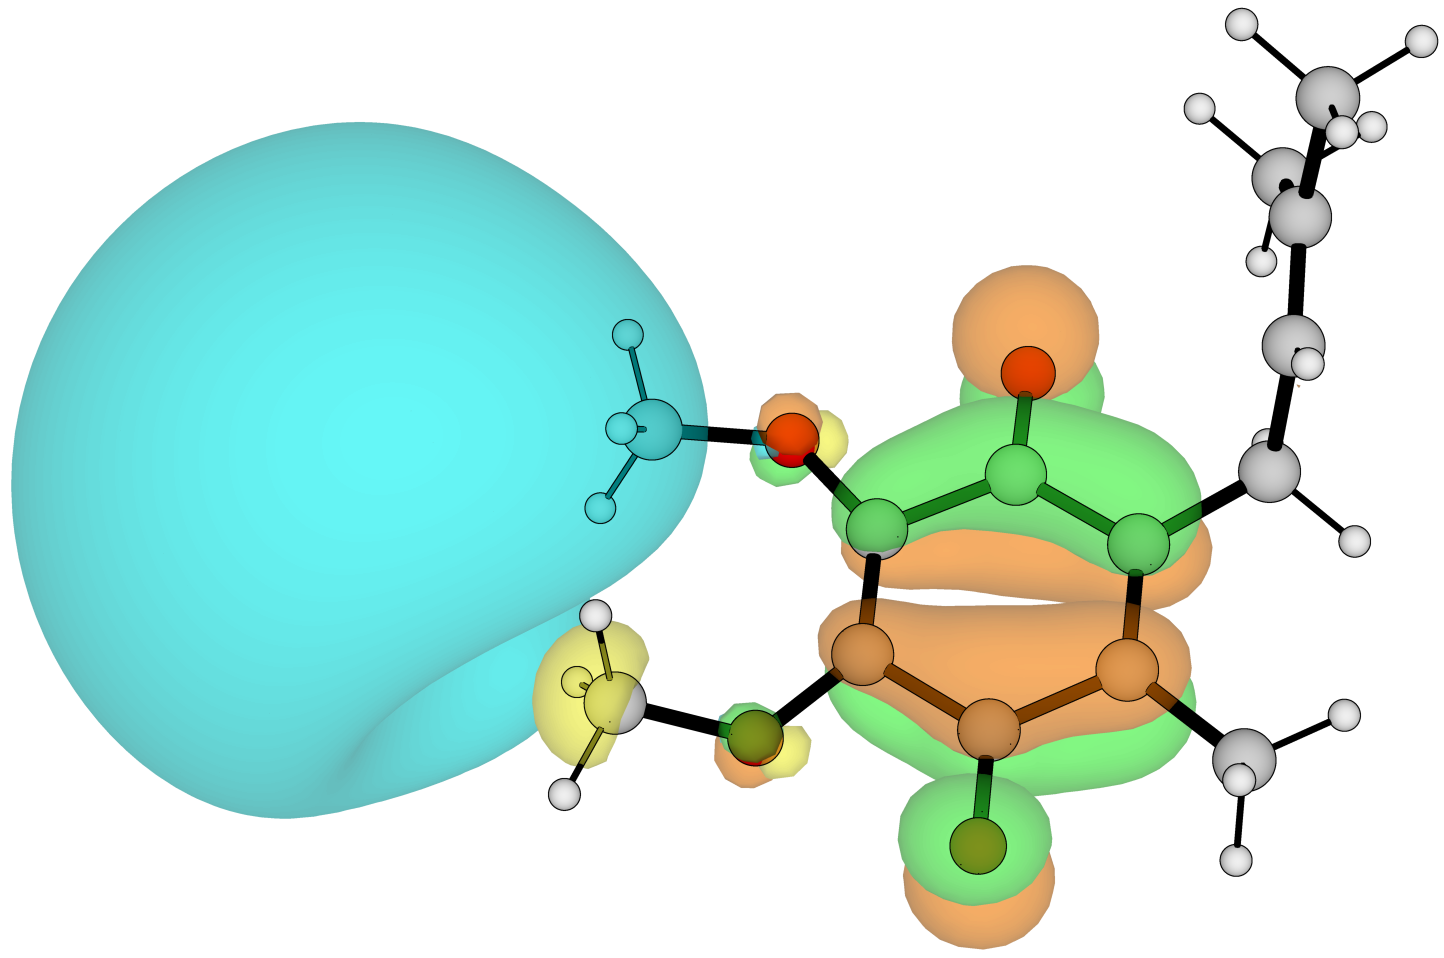
\includegraphics[width=0.6\textwidth]{Figs/Q1_cover.png}}
\end{frame}

\begin{frame}{\huge Overview}
\tableofcontents
\end{frame}

\section{Introduction}
\subsection{Non-valence anions}
\begin{frame}{\huge Non-valence anions}\large
    \vspace{5pt}
	The excess electron is bound by long-range forces (e.g., dipole, quadrupole). The `extra' electron density is located far from the molecule\\
	Found in atmospheric, interstellar, and biological environments; they act as `doorway' states for electron attachment
    \begin{itemize} 

            \item Extremely diffuse electron clouds
            \item Sensitive to correlation and environmental effects
            %\item Difficult to describe theoretically
            \item Require huge basis sets and accurate correlation treatment
    \end{itemize}
    \vspace{5pt}
	\begin{columns}
		\begin{column}{0.27\textwidth}
			\centering
			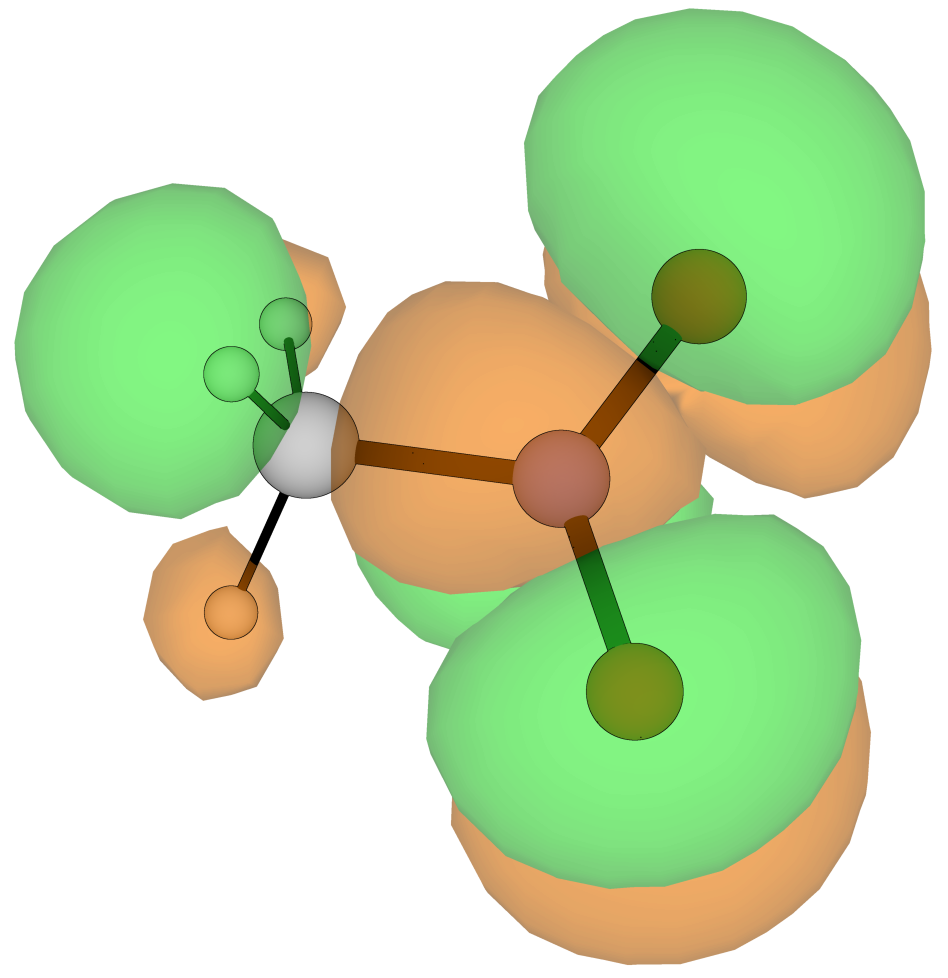
\includegraphics[width=0.55\textwidth]{Figs/MeNO2_VBS.png}\\
			\vspace{3pt}
			\small Valence-bound anion of nitromethane
		\end{column}
		\begin{column}{0.3\textwidth}
			\centering
			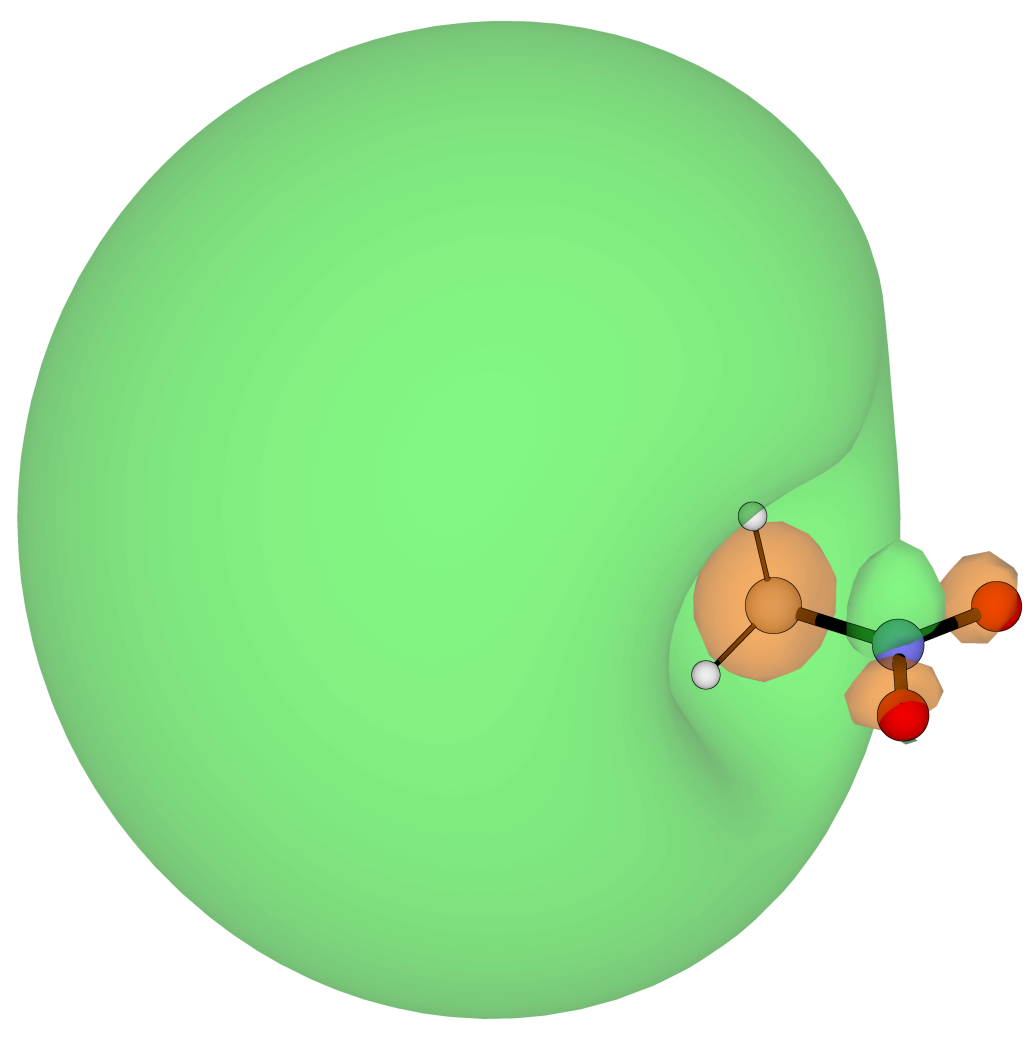
\includegraphics[width=0.55\textwidth]{Figs/MeNO2_DBS.png}\\
			\vspace{3pt}
    		\small Dipole-bound anion of nitromethane
		\end{column}
		\begin{column}{0.27\textwidth}
			\centering
			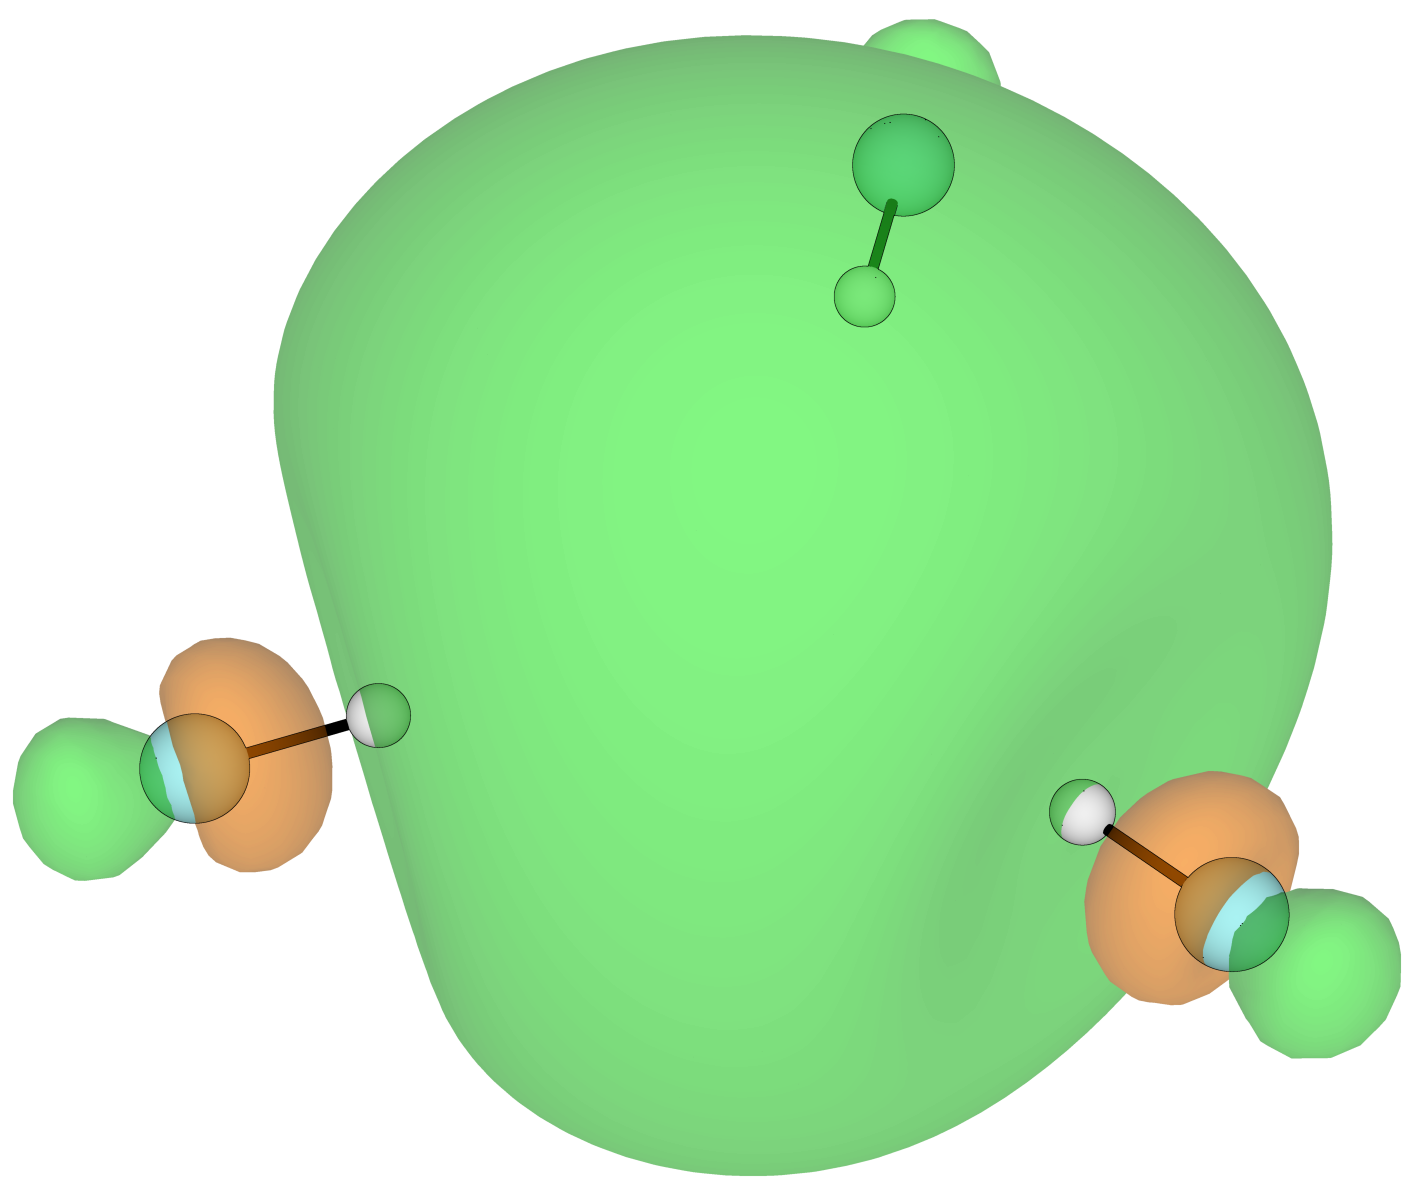
\includegraphics[width=0.7\textwidth]{Figs/hf3.png}\\
			\vspace{3pt}
			\small (HF)\textsubscript{3} solvated electron
		\end{column}	
	\end{columns}
\end{frame}

\subsection{Ubiquinone}
\begin{frame}{\huge Biological Quinones: Ubiquinone (CoQ)}\large
	Quinones are essential electron carriers in biological processes
		\vspace{5pt}
		\begin{itemize}
		%	\item Ubiquinone (coenzyme Q or CoQ) is a component of electron transport chains in bacterial photosynthesis and aerobic respiration.
		\item Component of electron transport chains in bacterial photosynthesis and aerobic respiration	
		\item Capable of both valence and dipole bound anion states
		\end{itemize}
		\begin{columns}[b]
			\begin{column}[b]{0.5\textwidth}
				\centering
				\includegraphics[width=0.8\textwidth]{Figs/Mitochondrial_electron_transport_chain—Etc4.svg.png}\\
				%\vspace{3pt}
				\small Mitochondrial Electron Transport Chain\\
				\footnotesize Source: Wikimedia Commons
			\end{column}
			\begin{column}[b]{0.25\textwidth}
				\centering
				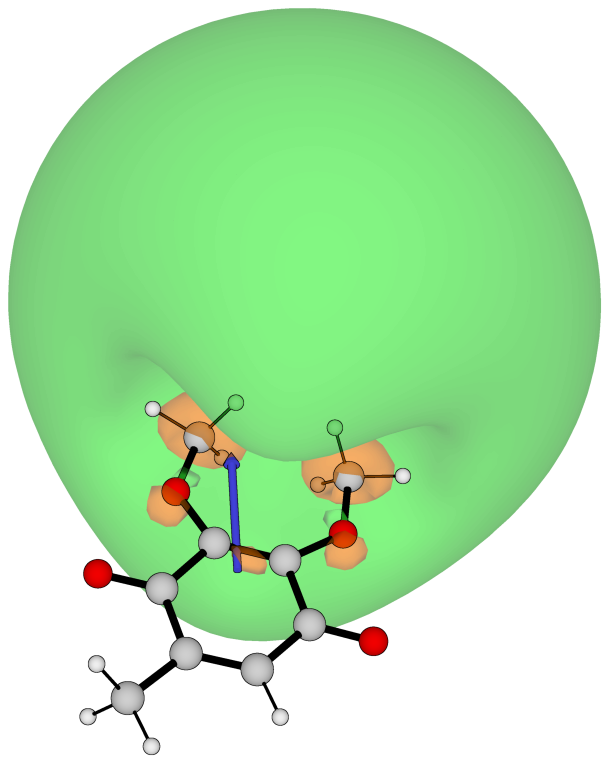
\includegraphics[width=0.9\textwidth]{Figs/Q0_181.png}\\
				\vspace{10pt}
				\small Dipole-bound state\\
				\footnotesize \vspace{\baselineskip}
			\end{column}
			\begin{column}[b]{0.25\textwidth}
				\centering
				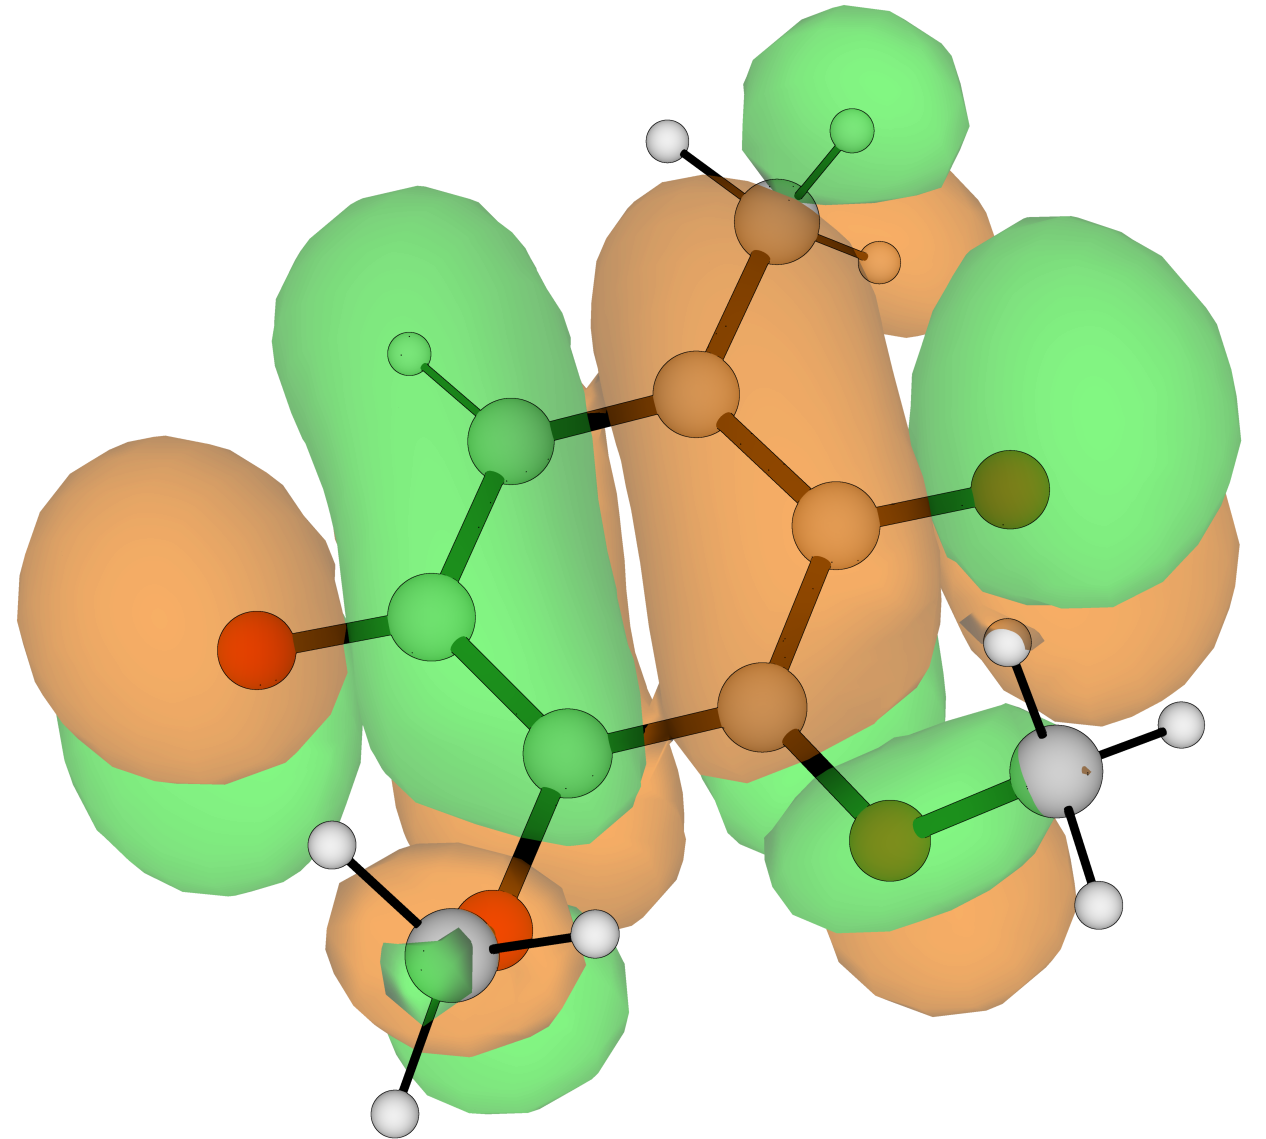
\includegraphics[width=1\textwidth]{Figs/Q0_52_VBS.png}\\
				\vspace{25pt}
				\small Valence-bound state\\
				\footnotesize \vspace{\baselineskip}
			\end{column}
		\end{columns}
\end{frame}

\begin{frame}{\huge Ubiquinone Structure}\large
	Each part of the molecule plays a distinct function:
	\begin{itemize}
		\item Quinone head involved in the electron transfer
		\item Isoprenoid tail responsible for the solubility in the membrane
		\item Methoxy chains determine the dipole moment
	\end{itemize}
	\vspace{130pt}
	\begin{columns}[b]
			\begin{column}{0.25\textwidth}
				\centering
				\Put(-70,150){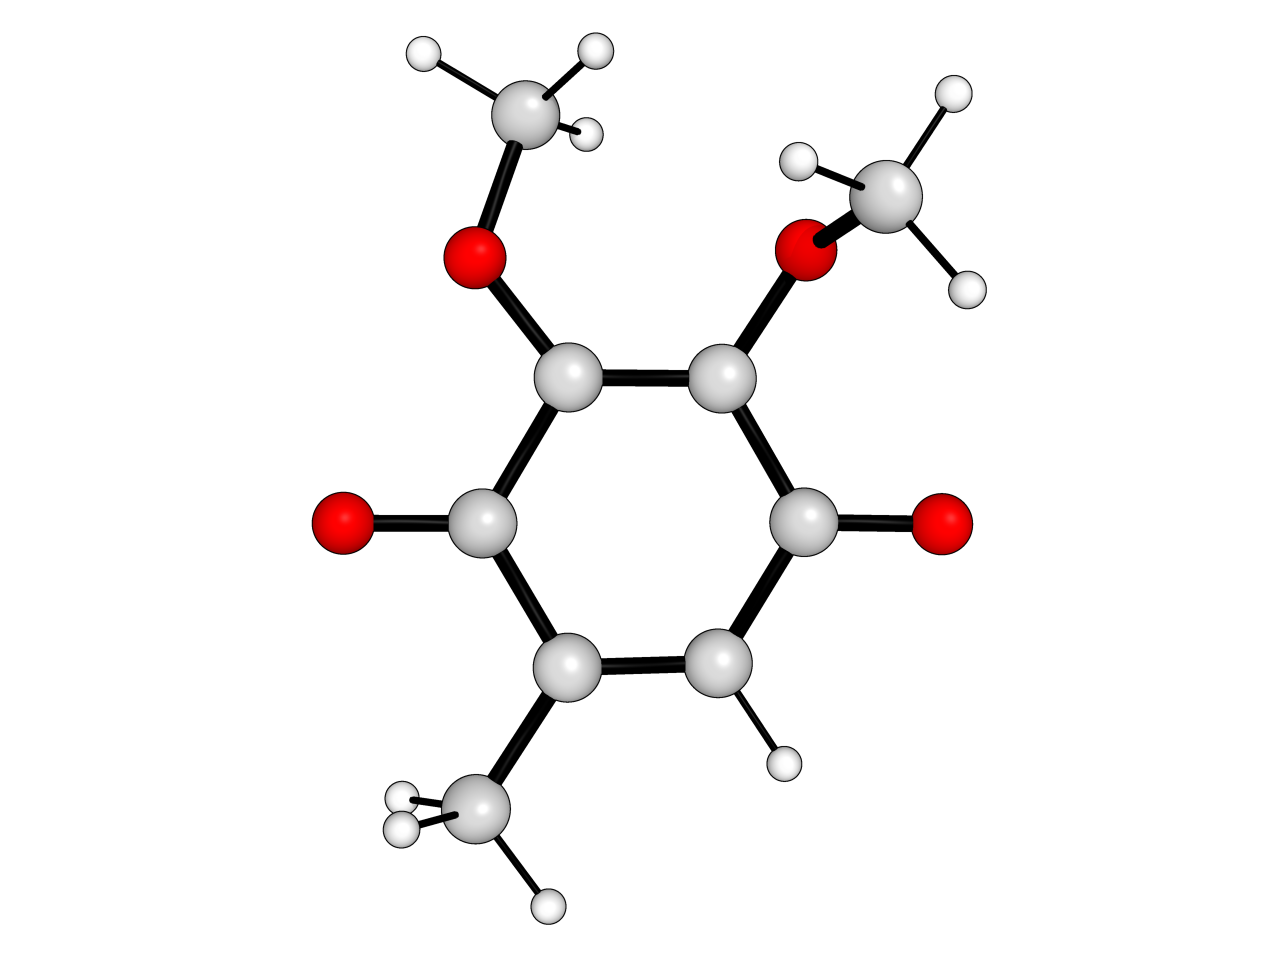
\includegraphics[width=1.6\textwidth]{Figs/Q0189.png}}
				Q\textsubscript{0}
			\end{column}
			\begin{column}{0.25\textwidth}
				\centering
				\Put(-80,150){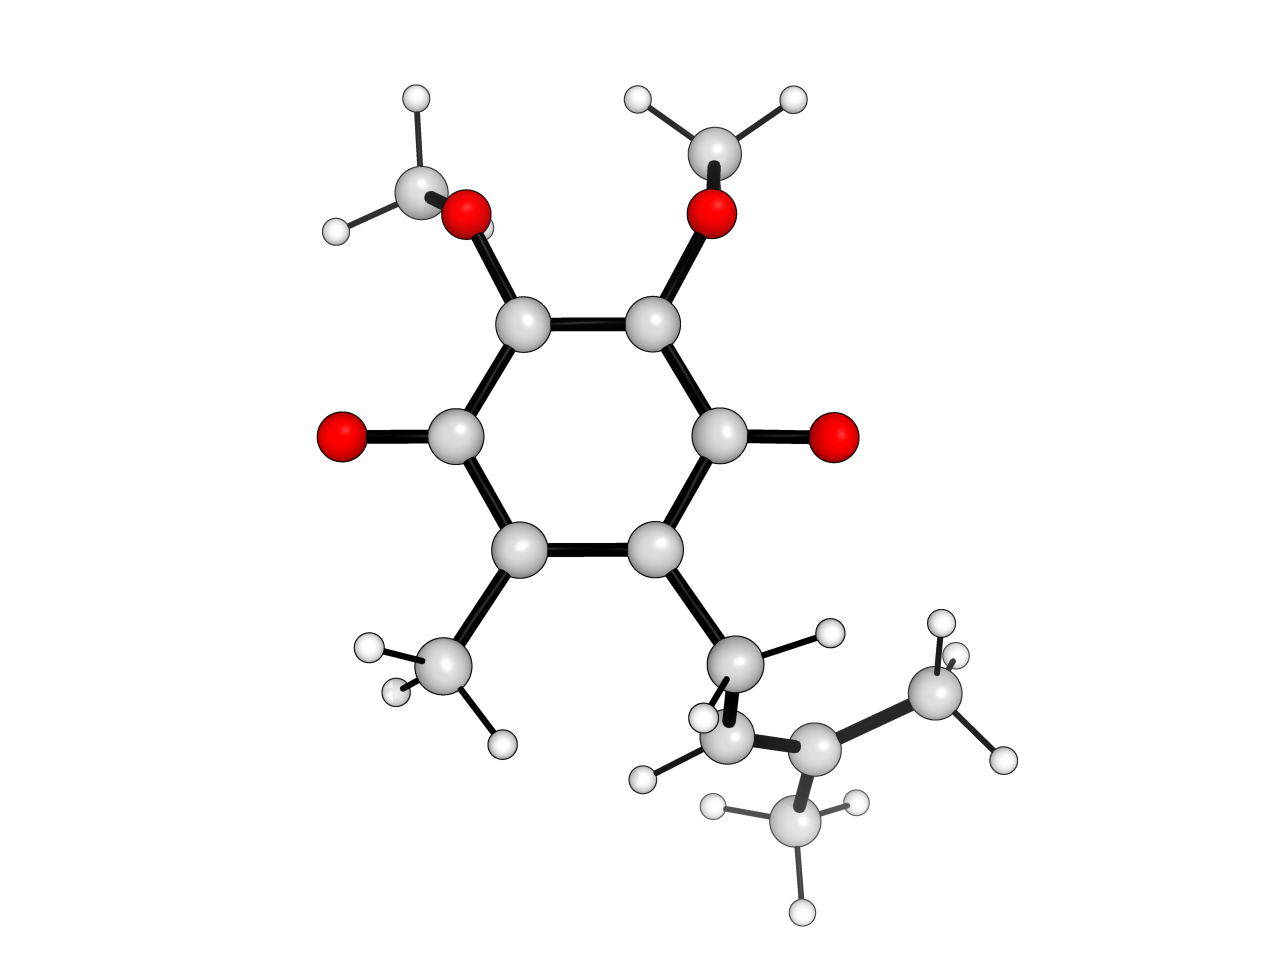
\includegraphics[width=1.8\textwidth]{Figs/Q1.png}}
				Q\textsubscript{1}
			\end{column}
			\begin{column}{0.4\textwidth}
				\centering
				\Put(-90,220){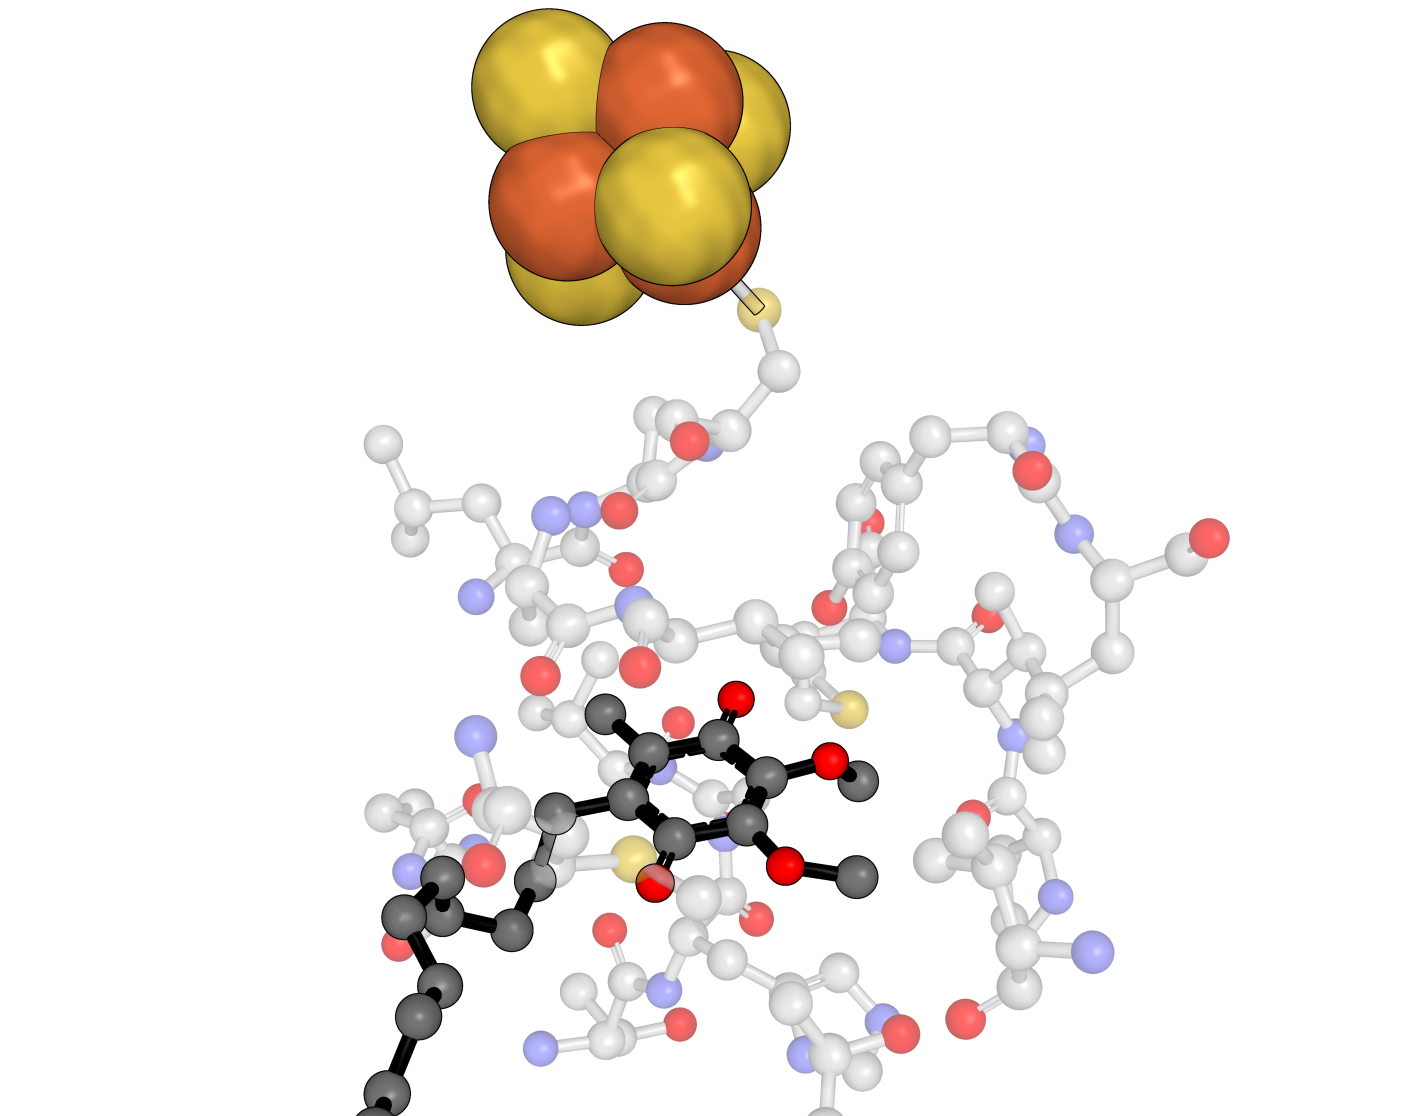
\includegraphics[width=1.4\textwidth]{Figs/uQ_6i0d.png}}
				Q\textsubscript{10} (PDB: 6I0D)
			\end{column}
		\end{columns}
\end{frame}

\section{Theory}

\subsection{Second-Order Approximate Coupled Cluster}
\begin{frame}{\huge CC2}\large
	Second-order approximate coupled-cluster singles and doubles (CC2) method is obtained from a perturbative analysis of the CCSD model
	\vspace{4pt}
	\begin{itemize}
		\item Doubles amplitudes are identical to MP2, singles are treated exactly
		\item Lowers computational scaling from CCSD: $O(N^5)$ vs. $O(N^6)$
		\item Allows treatment of “big” molecules: $>$ 25 heavy atoms
	\end{itemize}
	\vspace{5pt}
	\begin{columns}[c]
		\begin{column}{0.55\textwidth}
			\centering
			\[ |\Psi_{\mathrm{CC2}} \rangle = e^{\hat{T}_{\mathrm{CC2}}} | \Psi_0 \rangle \]
			\vspace{5pt}
			\[
			\hat{T}_{\mathrm{CC2}} = 1 + \sum_{ai} t^a a_a^\dagger a_i + \frac{1}{2} \sum_{ab} \sum_{ij} t_{ij}^{ab} a_a^\dagger a_b^\dagger a_j a_i  \] 
			\vspace{5pt}
			\[ t^{ab}_{ij} = \frac{1}{1+\delta_{ij}\delta_{ab}}\frac{\langle \phi_a \phi_b || \phi_i \phi_j \rangle}{\epsilon_a + \epsilon_b - \epsilon_i - \epsilon_j}
			\]
		\end{column}
		\begin{column}{0.45\textwidth}
			\begin{table}
				\centering
				\begin{tabular}{lcc}\toprule
				\textbf{Method} & \textbf{Scaling} & \textbf{Memory}\\\midrule
				CCSD & $O(N^6)$ & $O(N^{4})$\\
				CC2 & $O(N^5)$ & $O(N^{4})^*$\\\bottomrule
				\multicolumn{3}{l}{\small $^*\,O(N^3)$ with RI approximation.}
				\end{tabular}
			\end{table}
		\end{column}
	\end{columns}
	\vfill
\end{frame}

\subsection{Equation-of-Motion Electron-Attachment}
\begin{frame}{\huge EOM-EA}\large
	\begin{flushleft}
    Equation-of-motion electron-attachment coupled-cluster (EOM-EA-CC) methods are particularly well suited to study non-valence anions.
	The description is based on the wave function of the parent neutral molecule
	\end{flushleft}
	\centering
	\vspace{-2pt}
	    \[ |\Psi_{\mathrm{EA}} \rangle = \hat{R}_{\mathrm{EA}} | \Psi_0 \rangle \]
	\vspace{1pt}
		\[ \hat{R}_{\mathrm{EA}} = \sum_{a} r^a a_a^\dagger + \frac{1}{2} \sum_{ab} \sum_{i} r_{i}^{ab} a_a^\dagger a_i a_b^\dagger + \dots \]
	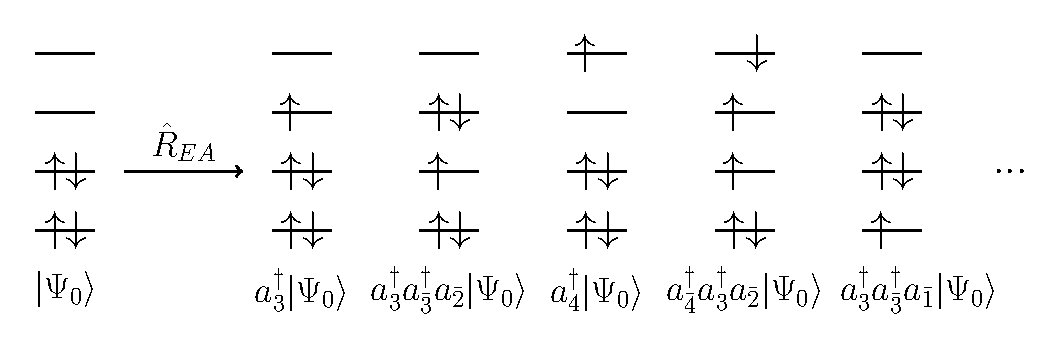
\includegraphics[width=0.8\textwidth]{Figs/EOM_EA.pdf}
	\vspace{3pt}
\end{frame}

\section{Computational Methods}
\begin{frame}{\huge Computational methods}\large
	All calculations were performed using the \textit{Q-Chem} software.
	\begin{itemize}
		\item Optimizations performed at TPSS+D3BJ/ma-def2-TZVP
		EA calculated at the RI-EOM-EA-CC2 using the neutral ground state as CC reference state
		\item aug-cc-pVDZ basis further augmented by 3 s-shells on hydrogen atoms and 6 s- and 3 p-shells on all non-hydrogen atoms
		\item Dyson orbitals calculated at the RI-EOM-EA-CC2 level (implemented in this thesis)
	\end{itemize}
	\vfill
	\centering
	%
\includegraphics[width=0.5\textwidth]{Figs/QCLogo.png}
	\vfill
\end{frame}

\section{Results}

\subsection{Methoxy chains rotation}
\begin{frame}{\huge Potential Energy Surface}\large
	We can construct surfaces from the methoxy rotations ($\Psi$ and $\Phi$) of the Q0 model.
	\begin{itemize}
		\item PES is constructed by scanning the dihedral angles $\Phi$ and $\Psi$ and visualized as a 2D map
		\item Rest of the molecule, which is quite rigid, is optimized at each point
	\end{itemize}
	\vspace{-20pt}
	\begin{columns}[c]
		\begin{column}{0.5\textwidth}
			\centering
			% GNUPLOT: LaTeX picture with Postscript
\begingroup
  \makeatletter
  \providecommand\color[2][]{%
    \GenericError{(gnuplot) \space\space\space\@spaces}{%
      Package color not loaded in conjunction with
      terminal option `colourtext'%
    }{See the gnuplot documentation for explanation.%
    }{Either use 'blacktext' in gnuplot or load the package
      color.sty in LaTeX.}%
    \renewcommand\color[2][]{}%
  }%
  \providecommand\includegraphics[2][]{%
    \GenericError{(gnuplot) \space\space\space\@spaces}{%
      Package graphicx or graphics not loaded%
    }{See the gnuplot documentation for explanation.%
    }{The gnuplot epslatex terminal needs graphicx.sty or graphics.sty.}%
    \renewcommand\includegraphics[2][]{}%
  }%
  \providecommand\rotatebox[2]{#2}%
  \@ifundefined{ifGPcolor}{%
    \newif\ifGPcolor
    \GPcolortrue
  }{}%
  \@ifundefined{ifGPblacktext}{%
    \newif\ifGPblacktext
    \GPblacktexttrue
  }{}%
  % define a \g@addto@macro without @ in the name:
  \let\gplgaddtomacro\g@addto@macro
  % define empty templates for all commands taking text:
  \gdef\gplbacktext{}%
  \gdef\gplfronttext{}%
  \makeatother
  \ifGPblacktext
    % no textcolor at all
    \def\colorrgb#1{}%
    \def\colorgray#1{}%
  \else
    % gray or color?
    \ifGPcolor
      \def\colorrgb#1{\color[rgb]{#1}}%
      \def\colorgray#1{\color[gray]{#1}}%
      \expandafter\def\csname LTw\endcsname{\color{white}}%
      \expandafter\def\csname LTb\endcsname{\color{black}}%
      \expandafter\def\csname LTa\endcsname{\color{black}}%
      \expandafter\def\csname LT0\endcsname{\color[rgb]{1,0,0}}%
      \expandafter\def\csname LT1\endcsname{\color[rgb]{0,1,0}}%
      \expandafter\def\csname LT2\endcsname{\color[rgb]{0,0,1}}%
      \expandafter\def\csname LT3\endcsname{\color[rgb]{1,0,1}}%
      \expandafter\def\csname LT4\endcsname{\color[rgb]{0,1,1}}%
      \expandafter\def\csname LT5\endcsname{\color[rgb]{1,1,0}}%
      \expandafter\def\csname LT6\endcsname{\color[rgb]{0,0,0}}%
      \expandafter\def\csname LT7\endcsname{\color[rgb]{1,0.3,0}}%
      \expandafter\def\csname LT8\endcsname{\color[rgb]{0.5,0.5,0.5}}%
    \else
      % gray
      \def\colorrgb#1{\color{black}}%
      \def\colorgray#1{\color[gray]{#1}}%
      \expandafter\def\csname LTw\endcsname{\color{white}}%
      \expandafter\def\csname LTb\endcsname{\color{black}}%
      \expandafter\def\csname LTa\endcsname{\color{black}}%
      \expandafter\def\csname LT0\endcsname{\color{black}}%
      \expandafter\def\csname LT1\endcsname{\color{black}}%
      \expandafter\def\csname LT2\endcsname{\color{black}}%
      \expandafter\def\csname LT3\endcsname{\color{black}}%
      \expandafter\def\csname LT4\endcsname{\color{black}}%
      \expandafter\def\csname LT5\endcsname{\color{black}}%
      \expandafter\def\csname LT6\endcsname{\color{black}}%
      \expandafter\def\csname LT7\endcsname{\color{black}}%
      \expandafter\def\csname LT8\endcsname{\color{black}}%
    \fi
  \fi
    \setlength{\unitlength}{0.0500bp}%
    \ifx\gptboxheight\undefined%
      \newlength{\gptboxheight}%
      \newlength{\gptboxwidth}%
      \newsavebox{\gptboxtext}%
    \fi%
    \setlength{\fboxrule}{0.5pt}%
    \setlength{\fboxsep}{1pt}%
    \definecolor{tbcol}{rgb}{1,1,1}%
\begin{picture}(3680.00,3680.00)%
    \gplgaddtomacro\gplbacktext{%
      \csname LTb\endcsname%%
      \put(714,959){\makebox(0,0)[r]{\strut{}$-150$}}%
      \csname LTb\endcsname%%
      \put(714,1314){\makebox(0,0)[r]{\strut{}$-100$}}%
      \csname LTb\endcsname%%
      \put(714,1668){\makebox(0,0)[r]{\strut{}$-50$}}%
      \csname LTb\endcsname%%
      \put(714,2023){\makebox(0,0)[r]{\strut{}$0$}}%
      \csname LTb\endcsname%%
      \put(714,2378){\makebox(0,0)[r]{\strut{}$50$}}%
      \csname LTb\endcsname%%
      \put(714,2732){\makebox(0,0)[r]{\strut{}$100$}}%
      \csname LTb\endcsname%%
      \put(714,3087){\makebox(0,0)[r]{\strut{}$150$}}%
      \csname LTb\endcsname%%
      \put(812,570){\makebox(0,0){\strut{}$-180$}}%
      \csname LTb\endcsname%%
      \put(1237,570){\makebox(0,0){\strut{}$-120$}}%
      \csname LTb\endcsname%%
      \put(1663,570){\makebox(0,0){\strut{}$-60$}}%
      \csname LTb\endcsname%%
      \put(2089,570){\makebox(0,0){\strut{}$0$}}%
      \csname LTb\endcsname%%
      \put(2514,570){\makebox(0,0){\strut{}$60$}}%
      \csname LTb\endcsname%%
      \put(2940,570){\makebox(0,0){\strut{}$120$}}%
      \csname LTb\endcsname%%
      \put(3366,570){\makebox(0,0){\strut{}$180$}}%
    }%
    \gplgaddtomacro\gplfronttext{%
      \csname LTb\endcsname%%
      \put(357,2023){\rotatebox{-270.00}{\makebox(0,0){\normalsize $\Psi$}}}%
      \csname LTb\endcsname%%
      \put(2089,306){\makebox(0,0){\normalsize $\Phi$}}%
      \csname LTb\endcsname%%
      \put(1770,2270){\rotatebox{-65.00}{\makebox(0,0){\strut{}\textcolor{black}{\footnotesize 500}}}}%
      \csname LTb\endcsname%%
      \put(2378,2036){\rotatebox{127.00}{\makebox(0,0){\strut{}\textcolor{black}{\footnotesize 400}}}}%
      \csname LTb\endcsname%%
      \put(1783,1948){\rotatebox{-45.00}{\makebox(0,0){\strut{}\textcolor{black}{\footnotesize 400}}}}%
      \csname LTb\endcsname%%
      \put(2029,2484){\rotatebox{152.00}{\makebox(0,0){\strut{}\textcolor{black}{\footnotesize 300}}}}%
      \csname LTb\endcsname%%
      \put(1885,1759){\rotatebox{-38.00}{\makebox(0,0){\strut{}\textcolor{black}{\footnotesize 300}}}}%
      \csname LTb\endcsname%%
      \put(2670,1883){\rotatebox{110.00}{\makebox(0,0){\strut{}\textcolor{black}{\footnotesize 200}}}}%
      \csname LTb\endcsname%%
      \put(1477,2794){\rotatebox{-167.00}{\makebox(0,0){\strut{}\textcolor{black}{\footnotesize 200}}}}%
      \csname LTb\endcsname%%
      \put(2014,1527){\rotatebox{-32.00}{\makebox(0,0){\strut{}\textcolor{black}{\footnotesize 200}}}}%
      \csname LTb\endcsname%%
      \put(1196,2849){\rotatebox{33.00}{\makebox(0,0){\strut{}\textcolor{black}{\footnotesize 100}}}}%
      \csname LTb\endcsname%%
      \put(2481,2849){\rotatebox{51.00}{\makebox(0,0){\strut{}\textcolor{black}{\footnotesize 100}}}}%
      \csname LTb\endcsname%%
      \put(2699,2098){\rotatebox{-73.00}{\makebox(0,0){\strut{}\textcolor{black}{\footnotesize 100}}}}%
      \csname LTb\endcsname%%
      \put(1241,2426){\rotatebox{-30.00}{\makebox(0,0){\strut{}\textcolor{black}{\footnotesize 100}}}}%
      \csname LTb\endcsname%%
      \put(1284,1230){\rotatebox{-38.00}{\makebox(0,0){\strut{}\textcolor{black}{\footnotesize 100}}}}%
      \csname LTb\endcsname%%
      \put(2572,1068){\rotatebox{-46.00}{\makebox(0,0){\strut{}\textcolor{black}{\footnotesize 100}}}}%
      \csname LTb\endcsname%%
      \put(962,2336){\rotatebox{-155.00}{\makebox(0,0){\strut{}\textcolor{black}{\footnotesize 50}}}}%
      \csname LTb\endcsname%%
      \put(2958,2287){\rotatebox{-162.00}{\makebox(0,0){\strut{}\textcolor{black}{\footnotesize 50}}}}%
      \csname LTb\endcsname%%
      \put(1820,2873){\rotatebox{-46.00}{\makebox(0,0){\strut{}\textcolor{black}{\footnotesize 50}}}}%
      \csname LTb\endcsname%%
      \put(1885,1197){\rotatebox{49.00}{\makebox(0,0){\strut{}\textcolor{black}{\footnotesize 50}}}}%
    }%
    \gplbacktext
    \put(0,0){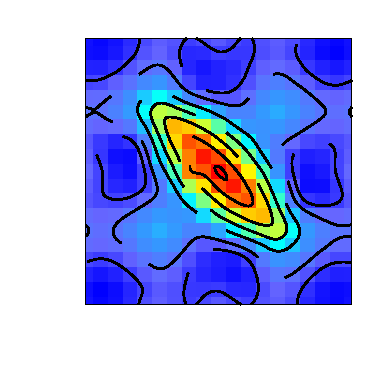
\includegraphics[width={184.00bp},height={184.00bp}]{Figs/Q0_E}}%
    \gplfronttext
  \end{picture}%
\endgroup

		\end{column}
		\begin{column}{0.5\textwidth}
			\centering
			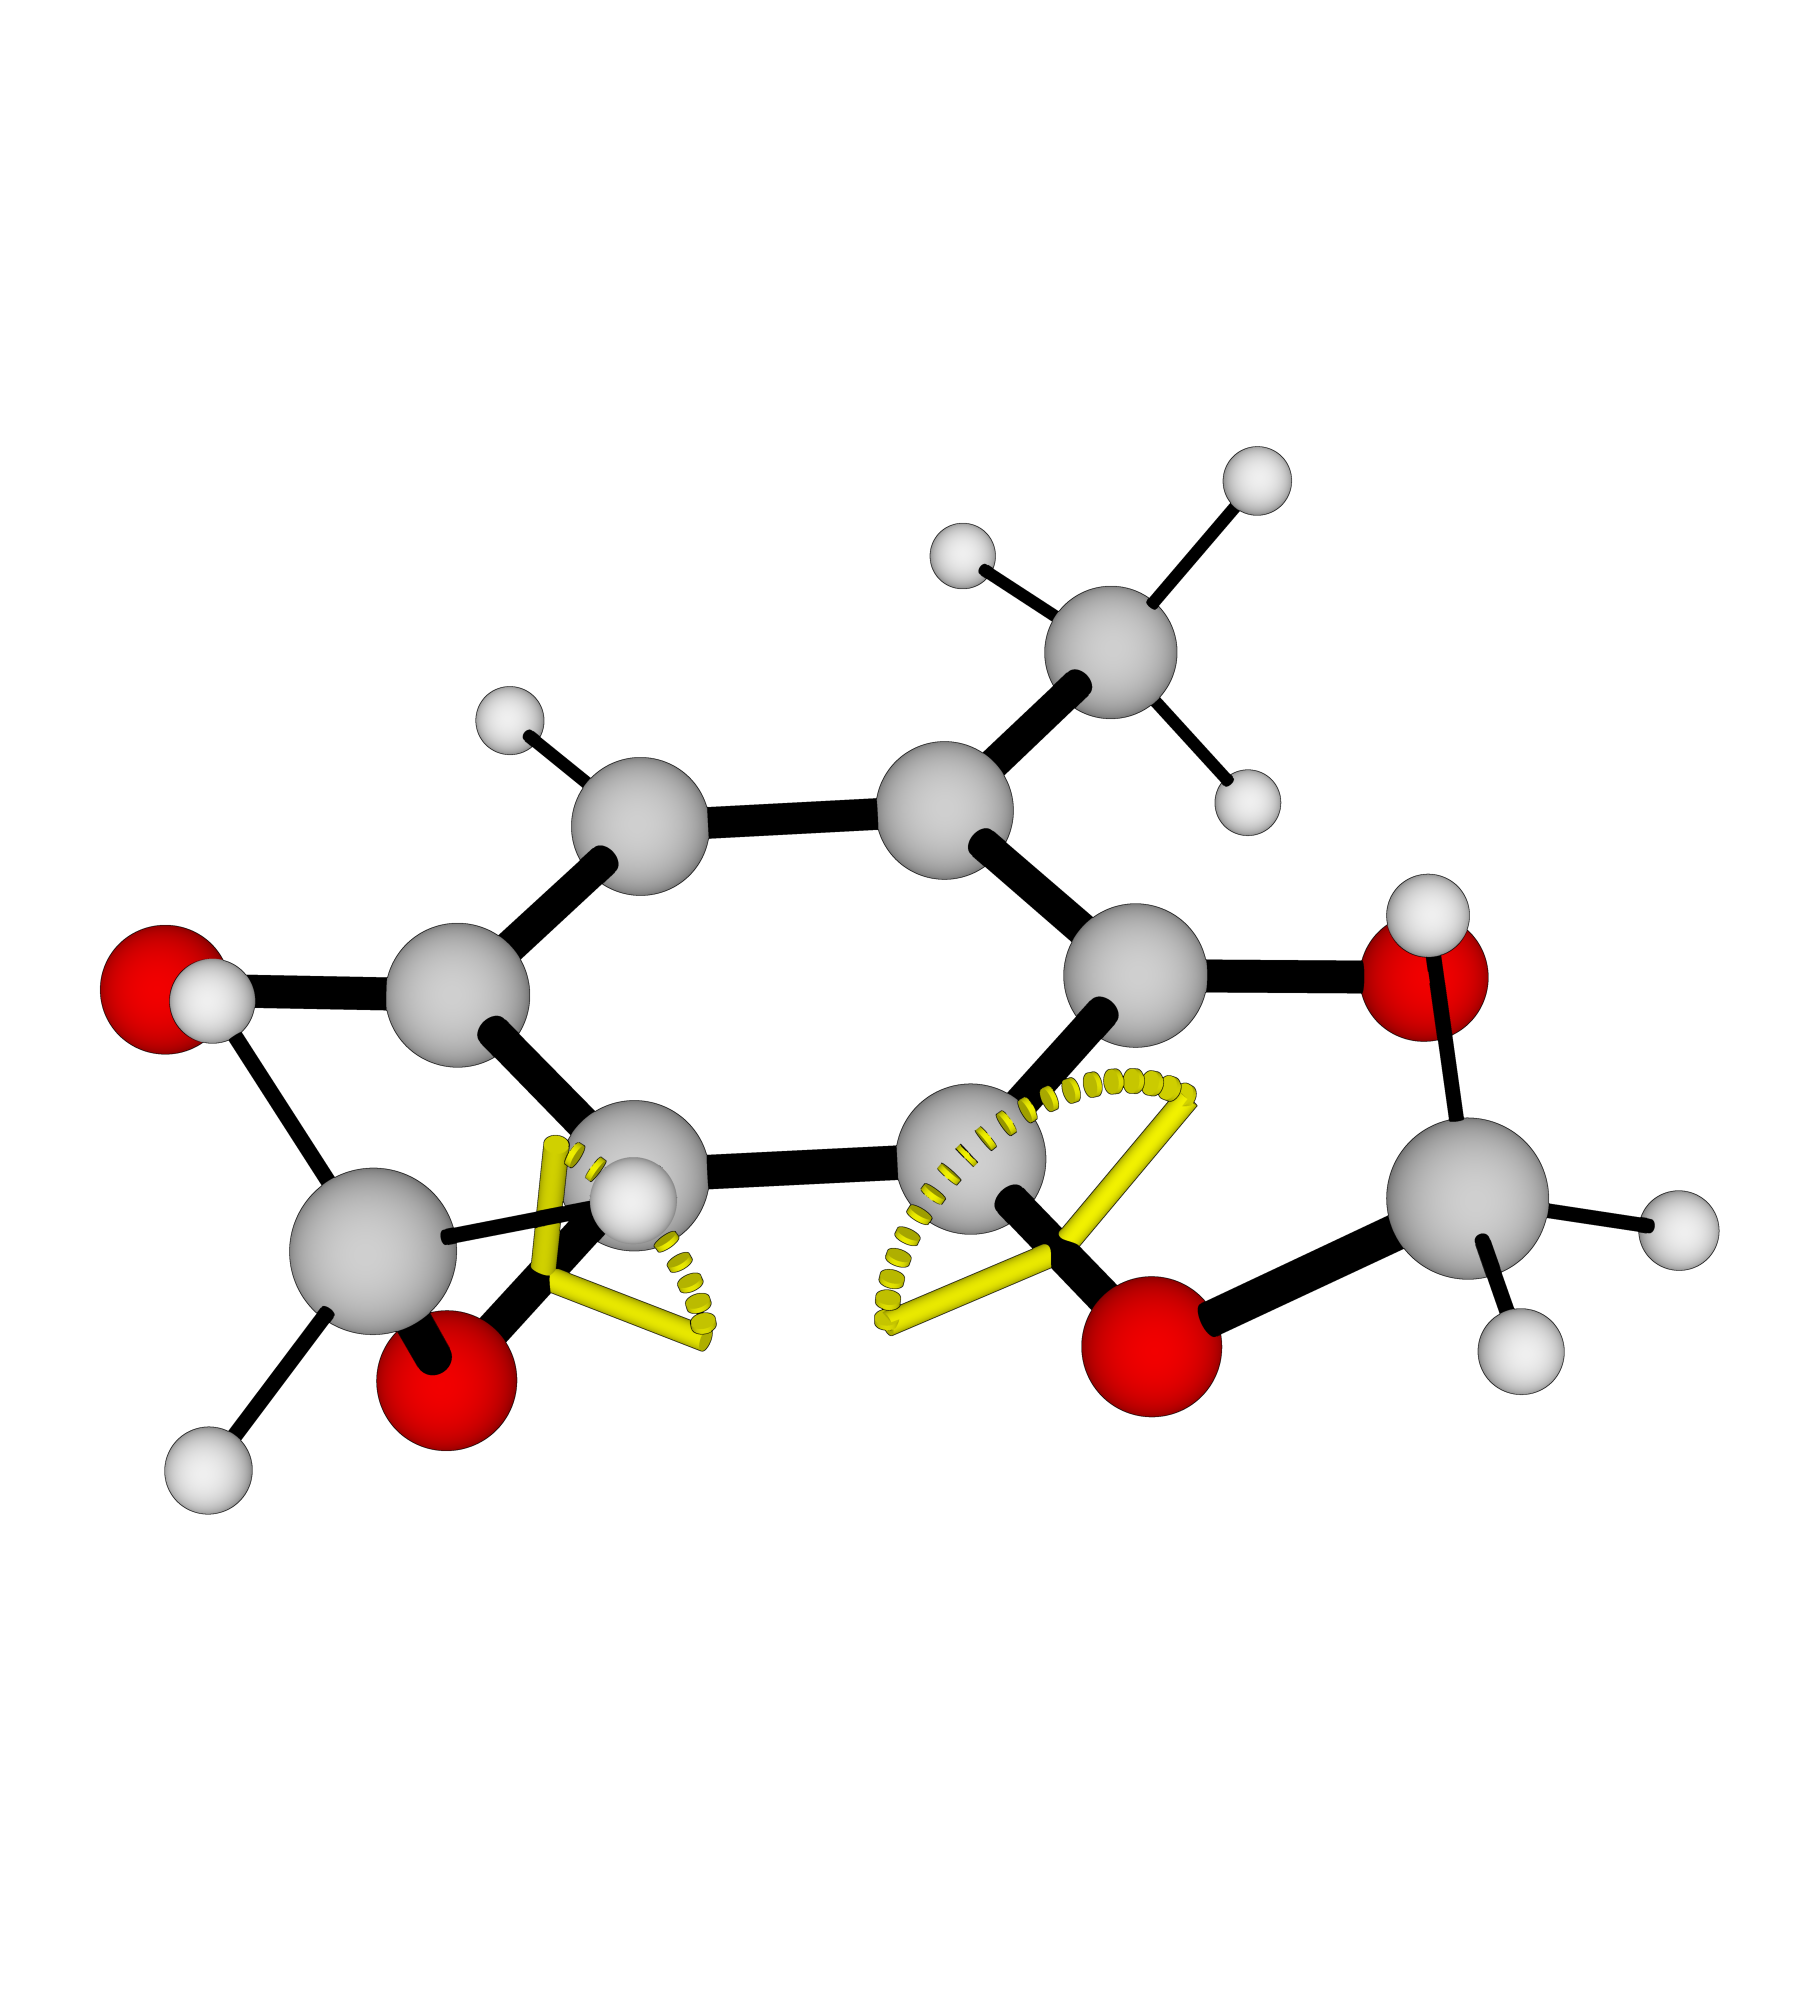
\includegraphics[width=0.9\textwidth]{Figs/dihedrals.png}
			\put(-160,40){\textbf{\large \textcolor{black}{$\mathrm{\Phi=80}\degree$}}}
			\put(-110,40){\textbf{\large \textcolor{black}{$\mathrm{\Psi=-140}\degree$}}}
		\end{column}
	\end{columns}
	\vspace{10pt}
\end{frame}

\begin{frame}{\huge Potential Energy Surfaces of Q0}\large
	\begin{columns}[t]
		\begin{column}{0.4\textwidth}
			\footnotesize
			\vspace{-22pt}
			% GNUPLOT: LaTeX picture with Postscript
\begingroup
  \makeatletter
  \providecommand\color[2][]{%
    \GenericError{(gnuplot) \space\space\space\@spaces}{%
      Package color not loaded in conjunction with
      terminal option `colourtext'%
    }{See the gnuplot documentation for explanation.%
    }{Either use 'blacktext' in gnuplot or load the package
      color.sty in LaTeX.}%
    \renewcommand\color[2][]{}%
  }%
  \providecommand\includegraphics[2][]{%
    \GenericError{(gnuplot) \space\space\space\@spaces}{%
      Package graphicx or graphics not loaded%
    }{See the gnuplot documentation for explanation.%
    }{The gnuplot epslatex terminal needs graphicx.sty or graphics.sty.}%
    \renewcommand\includegraphics[2][]{}%
  }%
  \providecommand\rotatebox[2]{#2}%
  \@ifundefined{ifGPcolor}{%
    \newif\ifGPcolor
    \GPcolortrue
  }{}%
  \@ifundefined{ifGPblacktext}{%
    \newif\ifGPblacktext
    \GPblacktexttrue
  }{}%
  % define a \g@addto@macro without @ in the name:
  \let\gplgaddtomacro\g@addto@macro
  % define empty templates for all commands taking text:
  \gdef\gplbacktext{}%
  \gdef\gplfronttext{}%
  \makeatother
  \ifGPblacktext
    % no textcolor at all
    \def\colorrgb#1{}%
    \def\colorgray#1{}%
  \else
    % gray or color?
    \ifGPcolor
      \def\colorrgb#1{\color[rgb]{#1}}%
      \def\colorgray#1{\color[gray]{#1}}%
      \expandafter\def\csname LTw\endcsname{\color{white}}%
      \expandafter\def\csname LTb\endcsname{\color{black}}%
      \expandafter\def\csname LTa\endcsname{\color{black}}%
      \expandafter\def\csname LT0\endcsname{\color[rgb]{1,0,0}}%
      \expandafter\def\csname LT1\endcsname{\color[rgb]{0,1,0}}%
      \expandafter\def\csname LT2\endcsname{\color[rgb]{0,0,1}}%
      \expandafter\def\csname LT3\endcsname{\color[rgb]{1,0,1}}%
      \expandafter\def\csname LT4\endcsname{\color[rgb]{0,1,1}}%
      \expandafter\def\csname LT5\endcsname{\color[rgb]{1,1,0}}%
      \expandafter\def\csname LT6\endcsname{\color[rgb]{0,0,0}}%
      \expandafter\def\csname LT7\endcsname{\color[rgb]{1,0.3,0}}%
      \expandafter\def\csname LT8\endcsname{\color[rgb]{0.5,0.5,0.5}}%
    \else
      % gray
      \def\colorrgb#1{\color{black}}%
      \def\colorgray#1{\color[gray]{#1}}%
      \expandafter\def\csname LTw\endcsname{\color{white}}%
      \expandafter\def\csname LTb\endcsname{\color{black}}%
      \expandafter\def\csname LTa\endcsname{\color{black}}%
      \expandafter\def\csname LT0\endcsname{\color{black}}%
      \expandafter\def\csname LT1\endcsname{\color{black}}%
      \expandafter\def\csname LT2\endcsname{\color{black}}%
      \expandafter\def\csname LT3\endcsname{\color{black}}%
      \expandafter\def\csname LT4\endcsname{\color{black}}%
      \expandafter\def\csname LT5\endcsname{\color{black}}%
      \expandafter\def\csname LT6\endcsname{\color{black}}%
      \expandafter\def\csname LT7\endcsname{\color{black}}%
      \expandafter\def\csname LT8\endcsname{\color{black}}%
    \fi
  \fi
    \setlength{\unitlength}{0.0500bp}%
    \ifx\gptboxheight\undefined%
      \newlength{\gptboxheight}%
      \newlength{\gptboxwidth}%
      \newsavebox{\gptboxtext}%
    \fi%
    \setlength{\fboxrule}{0.5pt}%
    \setlength{\fboxsep}{1pt}%
    \definecolor{tbcol}{rgb}{1,1,1}%
\begin{picture}(9060.00,9060.00)%
    \gplgaddtomacro\gplbacktext{%
    }%
    \gplgaddtomacro\gplfronttext{%
      \csname LTb\endcsname%%
      \put(444,5102){\makebox(0,0)[r]{\strut{}$-160$}}%
      \csname LTb\endcsname%%
      \put(444,5544){\makebox(0,0)[r]{\strut{}$-120$}}%
      \csname LTb\endcsname%%
      \put(444,5986){\makebox(0,0)[r]{\strut{}$-80$}}%
      \csname LTb\endcsname%%
      \put(444,6428){\makebox(0,0)[r]{\strut{}$-40$}}%
      \csname LTb\endcsname%%
      \put(444,6870){\makebox(0,0)[r]{\strut{}$0$}}%
      \csname LTb\endcsname%%
      \put(444,7312){\makebox(0,0)[r]{\strut{}$40$}}%
      \csname LTb\endcsname%%
      \put(444,7754){\makebox(0,0)[r]{\strut{}$80$}}%
      \csname LTb\endcsname%%
      \put(444,8196){\makebox(0,0)[r]{\strut{}$120$}}%
      \csname LTb\endcsname%%
      \put(444,8638){\makebox(0,0)[r]{\strut{}$160$}}%
      \csname LTb\endcsname%%
      \put(542,4705){\makebox(0,0){\strut{}}}%
      \csname LTb\endcsname%%
      \put(1205,4705){\makebox(0,0){\strut{}}}%
      \csname LTb\endcsname%%
      \put(1868,4705){\makebox(0,0){\strut{}}}%
      \csname LTb\endcsname%%
      \put(2531,4705){\makebox(0,0){\strut{}}}%
      \csname LTb\endcsname%%
      \put(3194,4705){\makebox(0,0){\strut{}}}%
      \csname LTb\endcsname%%
      \put(3857,4705){\makebox(0,0){\strut{}}}%
      \csname LTb\endcsname%%
      \put(4520,4705){\makebox(0,0){\strut{}}}%
      \csname LTb\endcsname%%
      \put(87,6870){\rotatebox{-270.00}{\makebox(0,0){\normalsize $\Psi$}}}%
      \csname LTb\endcsname%%
      \put(2089,7154){\rotatebox{-66.00}{\makebox(0,0){\strut{}\textcolor{black}{\footnotesize 500}}}}%
      \csname LTb\endcsname%%
      \put(2907,6987){\rotatebox{130.00}{\makebox(0,0){\strut{}\textcolor{black}{\footnotesize 400}}}}%
      \csname LTb\endcsname%%
      \put(2146,6682){\rotatebox{-27.00}{\makebox(0,0){\strut{}\textcolor{black}{\footnotesize 400}}}}%
      \csname LTb\endcsname%%
      \put(2313,7650){\rotatebox{154.00}{\makebox(0,0){\strut{}\textcolor{black}{\footnotesize 300}}}}%
      \csname LTb\endcsname%%
      \put(2302,6385){\rotatebox{-39.00}{\makebox(0,0){\strut{}\textcolor{black}{\footnotesize 300}}}}%
      \csname LTb\endcsname%%
      \put(3383,6779){\rotatebox{113.00}{\makebox(0,0){\strut{}\textcolor{black}{\footnotesize 200}}}}%
      \csname LTb\endcsname%%
      \put(1472,8023){\rotatebox{-143.00}{\makebox(0,0){\strut{}\textcolor{black}{\footnotesize 200}}}}%
      \csname LTb\endcsname%%
      \put(2514,6042){\rotatebox{-26.00}{\makebox(0,0){\strut{}\textcolor{black}{\footnotesize 200}}}}%
      \csname LTb\endcsname%%
      \put(1231,8224){\rotatebox{39.00}{\makebox(0,0){\strut{}\textcolor{black}{\footnotesize 100}}}}%
      \csname LTb\endcsname%%
      \put(3216,8239){\rotatebox{42.00}{\makebox(0,0){\strut{}\textcolor{black}{\footnotesize 100}}}}%
      \csname LTb\endcsname%%
      \put(3517,6877){\rotatebox{-71.00}{\makebox(0,0){\strut{}\textcolor{black}{\footnotesize 100}}}}%
      \csname LTb\endcsname%%
      \put(1307,7421){\rotatebox{-43.00}{\makebox(0,0){\strut{}\textcolor{black}{\footnotesize 100}}}}%
      \csname LTb\endcsname%%
      \put(1378,5563){\rotatebox{-33.00}{\makebox(0,0){\strut{}\textcolor{black}{\footnotesize 100}}}}%
      \csname LTb\endcsname%%
      \put(3383,5294){\rotatebox{-28.00}{\makebox(0,0){\strut{}\textcolor{black}{\footnotesize 100}}}}%
      \csname LTb\endcsname%%
      \put(705,7288){\rotatebox{-112.00}{\makebox(0,0){\strut{}\textcolor{black}{\footnotesize 50}}}}%
      \csname LTb\endcsname%%
      \put(3758,7221){\rotatebox{-149.00}{\makebox(0,0){\strut{}\textcolor{black}{\footnotesize 50}}}}%
      \csname LTb\endcsname%%
      \put(2213,8126){\rotatebox{-28.00}{\makebox(0,0){\strut{}\textcolor{black}{\footnotesize 50}}}}%
      \csname LTb\endcsname%%
      \put(2292,5650){\rotatebox{31.00}{\makebox(0,0){\strut{}\textcolor{black}{\footnotesize 50}}}}%
      \csname LTb\endcsname%%
      \put(2531,8982){\makebox(0,0){\strut{}Conformational Energy (meV)}}%
    }%
    \gplgaddtomacro\gplbacktext{%
    }%
    \gplgaddtomacro\gplfronttext{%
      \csname LTb\endcsname%%
      \put(4874,5102){\makebox(0,0)[r]{\strut{}}}%
      \csname LTb\endcsname%%
      \put(4874,5544){\makebox(0,0)[r]{\strut{}}}%
      \csname LTb\endcsname%%
      \put(4874,5986){\makebox(0,0)[r]{\strut{}}}%
      \csname LTb\endcsname%%
      \put(4874,6428){\makebox(0,0)[r]{\strut{}}}%
      \csname LTb\endcsname%%
      \put(4874,6870){\makebox(0,0)[r]{\strut{}}}%
      \csname LTb\endcsname%%
      \put(4874,7312){\makebox(0,0)[r]{\strut{}}}%
      \csname LTb\endcsname%%
      \put(4874,7754){\makebox(0,0)[r]{\strut{}}}%
      \csname LTb\endcsname%%
      \put(4874,8196){\makebox(0,0)[r]{\strut{}}}%
      \csname LTb\endcsname%%
      \put(4874,8638){\makebox(0,0)[r]{\strut{}}}%
      \csname LTb\endcsname%%
      \put(4971,4705){\makebox(0,0){\strut{}}}%
      \csname LTb\endcsname%%
      \put(5634,4705){\makebox(0,0){\strut{}}}%
      \csname LTb\endcsname%%
      \put(6297,4705){\makebox(0,0){\strut{}}}%
      \csname LTb\endcsname%%
      \put(6960,4705){\makebox(0,0){\strut{}}}%
      \csname LTb\endcsname%%
      \put(7623,4705){\makebox(0,0){\strut{}}}%
      \csname LTb\endcsname%%
      \put(8286,4705){\makebox(0,0){\strut{}}}%
      \csname LTb\endcsname%%
      \put(8949,4705){\makebox(0,0){\strut{}}}%
      \csname LTb\endcsname%%
      \put(5031,7851){\rotatebox{37.00}{\makebox(0,0){\strut{}\textcolor{black}{\footnotesize 3.0}}}}%
      \csname LTb\endcsname%%
      \put(8832,6500){\rotatebox{156.00}{\makebox(0,0){\strut{}\textcolor{black}{\footnotesize 3.0}}}}%
      \csname LTb\endcsname%%
      \put(6547,7260){\rotatebox{-78.00}{\makebox(0,0){\strut{}\textcolor{black}{\footnotesize 2.5}}}}%
      \csname LTb\endcsname%%
      \put(5651,8271){\rotatebox{-7.00}{\makebox(0,0){\strut{}\textcolor{black}{\footnotesize 2.5}}}}%
      \csname LTb\endcsname%%
      \put(5409,6940){\rotatebox{-127.00}{\makebox(0,0){\strut{}\textcolor{black}{\footnotesize 2.5}}}}%
      \csname LTb\endcsname%%
      \put(8618,7519){\rotatebox{-88.00}{\makebox(0,0){\strut{}\textcolor{black}{\footnotesize 2.5}}}}%
      \csname LTb\endcsname%%
      \put(8083,6140){\rotatebox{-101.00}{\makebox(0,0){\strut{}\textcolor{black}{\footnotesize 2.5}}}}%
      \csname LTb\endcsname%%
      \put(5500,6320){\rotatebox{91.00}{\makebox(0,0){\strut{}\textcolor{black}{\footnotesize 2.0}}}}%
      \csname LTb\endcsname%%
      \put(6314,7040){\rotatebox{-47.00}{\makebox(0,0){\strut{}\textcolor{black}{\footnotesize 2.0}}}}%
      \csname LTb\endcsname%%
      \put(7233,6000){\rotatebox{-38.00}{\makebox(0,0){\strut{}\textcolor{black}{\footnotesize 2.0}}}}%
      \csname LTb\endcsname%%
      \put(6531,7999){\rotatebox{-101.00}{\makebox(0,0){\strut{}\textcolor{black}{\footnotesize 2.0}}}}%
      \csname LTb\endcsname%%
      \put(7425,6960){\rotatebox{-59.00}{\makebox(0,0){\strut{}\textcolor{black}{\footnotesize 2.0}}}}%
      \csname LTb\endcsname%%
      \put(8359,7080){\rotatebox{64.00}{\makebox(0,0){\strut{}\textcolor{black}{\footnotesize 2.0}}}}%
      \csname LTb\endcsname%%
      \put(5471,5690){\rotatebox{52.00}{\makebox(0,0){\strut{}\textcolor{black}{\footnotesize 1.5}}}}%
      \csname LTb\endcsname%%
      \put(6291,6706){\rotatebox{-17.00}{\makebox(0,0){\strut{}\textcolor{black}{\footnotesize 1.5}}}}%
      \csname LTb\endcsname%%
      \put(6870,5426){\rotatebox{-106.00}{\makebox(0,0){\strut{}\textcolor{black}{\footnotesize 1.5}}}}%
      \csname LTb\endcsname%%
      \put(7650,8582){\rotatebox{-176.00}{\makebox(0,0){\strut{}\textcolor{black}{\footnotesize 1.5}}}}%
      \csname LTb\endcsname%%
      \put(7238,7519){\rotatebox{-45.00}{\makebox(0,0){\strut{}\textcolor{black}{\footnotesize 1.5}}}}%
      \csname LTb\endcsname%%
      \put(8205,7420){\rotatebox{78.00}{\makebox(0,0){\strut{}\textcolor{black}{\footnotesize 1.5}}}}%
      \csname LTb\endcsname%%
      \put(5771,5854){\rotatebox{56.00}{\makebox(0,0){\strut{}\textcolor{black}{\footnotesize 1.0}}}}%
      \csname LTb\endcsname%%
      \put(6570,5482){\rotatebox{-124.00}{\makebox(0,0){\strut{}\textcolor{black}{\footnotesize 1.0}}}}%
      \csname LTb\endcsname%%
      \put(7490,8350){\rotatebox{-162.00}{\makebox(0,0){\strut{}\textcolor{black}{\footnotesize 1.0}}}}%
      \csname LTb\endcsname%%
      \put(8062,7739){\rotatebox{60.00}{\makebox(0,0){\strut{}\textcolor{black}{\footnotesize 1.0}}}}%
      \csname LTb\endcsname%%
      \put(5883,5721){\rotatebox{-132.00}{\makebox(0,0){\strut{}\textcolor{black}{\footnotesize 0.5}}}}%
      \csname LTb\endcsname%%
      \put(7669,8179){\rotatebox{-140.00}{\makebox(0,0){\strut{}\textcolor{black}{\footnotesize 0.5}}}}%
      \csname LTb\endcsname%%
      \put(6960,8982){\makebox(0,0){Dipole Strength (Debye)}}%
    }%
    \gplgaddtomacro\gplbacktext{%
    }%
    \gplgaddtomacro\gplfronttext{%
      \csname LTb\endcsname%%
      \put(444,763){\makebox(0,0)[r]{\strut{}$-160$}}%
      \csname LTb\endcsname%%
      \put(444,1205){\makebox(0,0)[r]{\strut{}$-120$}}%
      \csname LTb\endcsname%%
      \put(444,1647){\makebox(0,0)[r]{\strut{}$-80$}}%
      \csname LTb\endcsname%%
      \put(444,2089){\makebox(0,0)[r]{\strut{}$-40$}}%
      \csname LTb\endcsname%%
      \put(444,2531){\makebox(0,0)[r]{\strut{}$0$}}%
      \csname LTb\endcsname%%
      \put(444,2973){\makebox(0,0)[r]{\strut{}$40$}}%
      \csname LTb\endcsname%%
      \put(444,3415){\makebox(0,0)[r]{\strut{}$80$}}%
      \csname LTb\endcsname%%
      \put(444,3857){\makebox(0,0)[r]{\strut{}$120$}}%
      \csname LTb\endcsname%%
      \put(444,4298){\makebox(0,0)[r]{\strut{}$160$}}%
      \csname LTb\endcsname%%
      \put(542,366){\makebox(0,0){\strut{}$-180$}}%
      \csname LTb\endcsname%%
      \put(1205,366){\makebox(0,0){\strut{}$-120$}}%
      \csname LTb\endcsname%%
      \put(1868,366){\makebox(0,0){\strut{}$-60$}}%
      \csname LTb\endcsname%%
      \put(2531,366){\makebox(0,0){\strut{}$0$}}%
      \csname LTb\endcsname%%
      \put(3194,366){\makebox(0,0){\strut{}$60$}}%
      \csname LTb\endcsname%%
      \put(3857,366){\makebox(0,0){\strut{}$120$}}%
      \csname LTb\endcsname%%
      \put(4519,366){\makebox(0,0){\strut{}$180$}}%
      \csname LTb\endcsname%%
      \put(87,2531){\rotatebox{-270.00}{\makebox(0,0){\normalsize $\Psi$}}}%
      \csname LTb\endcsname%%
      \put(2531,102){\makebox(0,0){\normalsize $\Phi$}}%
      \csname LTb\endcsname%%
      \put(2390,2781){\rotatebox{150.00}{\makebox(0,0){\strut{}\textcolor{black}{\footnotesize 1.3}}}}%
      \csname LTb\endcsname%%
      \put(2270,2355){\rotatebox{-57.00}{\makebox(0,0){\strut{}\textcolor{black}{\footnotesize 1.4}}}}%
      \csname LTb\endcsname%%
      \put(2912,2859){\rotatebox{124.00}{\makebox(0,0){\strut{}\textcolor{black}{\footnotesize 1.5}}}}%
      \csname LTb\endcsname%%
      \put(2511,1819){\rotatebox{-36.00}{\makebox(0,0){\strut{}\textcolor{black}{\footnotesize 1.5}}}}%
      \csname LTb\endcsname%%
      \put(2052,3555){\rotatebox{51.00}{\makebox(0,0){\strut{}\textcolor{black}{\footnotesize 1.6}}}}%
      \csname LTb\endcsname%%
      \put(2164,1627){\rotatebox{-79.00}{\makebox(0,0){\strut{}\textcolor{black}{\footnotesize 1.6}}}}%
      \csname LTb\endcsname%%
      \put(3435,2928){\rotatebox{-15.00}{\makebox(0,0){\strut{}\textcolor{black}{\footnotesize 1.6}}}}%
      \csname LTb\endcsname%%
      \put(3530,2028){\rotatebox{40.00}{\makebox(0,0){\strut{}\textcolor{black}{\footnotesize 1.6}}}}%
      \csname LTb\endcsname%%
      \put(1814,1426){\rotatebox{-81.00}{\makebox(0,0){\strut{}\textcolor{black}{\footnotesize 1.7}}}}%
      \csname LTb\endcsname%%
      \put(1753,3676){\rotatebox{49.00}{\makebox(0,0){\strut{}\textcolor{black}{\footnotesize 1.7}}}}%
      \csname LTb\endcsname%%
      \put(3475,3295){\rotatebox{-26.00}{\makebox(0,0){\strut{}\textcolor{black}{\footnotesize 1.7}}}}%
      \csname LTb\endcsname%%
      \put(3592,1667){\rotatebox{55.00}{\makebox(0,0){\strut{}\textcolor{black}{\footnotesize 1.7}}}}%
      \csname LTb\endcsname%%
      \put(2531,4643){\makebox(0,0){VBA EA (eV)}}%
    }%
    \gplgaddtomacro\gplbacktext{%
    }%
    \gplgaddtomacro\gplfronttext{%
      \csname LTb\endcsname%%
      \put(4874,763){\makebox(0,0)[r]{\strut{}}}%
      \csname LTb\endcsname%%
      \put(4874,1205){\makebox(0,0)[r]{\strut{}}}%
      \csname LTb\endcsname%%
      \put(4874,1647){\makebox(0,0)[r]{\strut{}}}%
      \csname LTb\endcsname%%
      \put(4874,2089){\makebox(0,0)[r]{\strut{}}}%
      \csname LTb\endcsname%%
      \put(4874,2531){\makebox(0,0)[r]{\strut{}}}%
      \csname LTb\endcsname%%
      \put(4874,2973){\makebox(0,0)[r]{\strut{}}}%
      \csname LTb\endcsname%%
      \put(4874,3415){\makebox(0,0)[r]{\strut{}}}%
      \csname LTb\endcsname%%
      \put(4874,3857){\makebox(0,0)[r]{\strut{}}}%
      \csname LTb\endcsname%%
      \put(4874,4298){\makebox(0,0)[r]{\strut{}}}%
      \csname LTb\endcsname%%
      \put(4971,366){\makebox(0,0){\strut{}$-180$}}%
      \csname LTb\endcsname%%
      \put(5634,366){\makebox(0,0){\strut{}$-120$}}%
      \csname LTb\endcsname%%
      \put(6297,366){\makebox(0,0){\strut{}$-60$}}%
      \csname LTb\endcsname%%
      \put(6960,366){\makebox(0,0){\strut{}$0$}}%
      \csname LTb\endcsname%%
      \put(7623,366){\makebox(0,0){\strut{}$60$}}%
      \csname LTb\endcsname%%
      \put(8286,366){\makebox(0,0){\strut{}$120$}}%
      \csname LTb\endcsname%%
      \put(8949,366){\makebox(0,0){\strut{}$180$}}%
      \csname LTb\endcsname%%
      \put(6960,102){\makebox(0,0){\normalsize $\Phi$}}%
      \csname LTb\endcsname%%
      \put(7021,2310){\rotatebox{-43.00}{\makebox(0,0){\strut{}\textcolor{black}{\footnotesize 12}}}}%
      \csname LTb\endcsname%%
      \put(7236,2069){\rotatebox{-30.00}{\makebox(0,0){\strut{}\textcolor{black}{\footnotesize 9}}}}%
      \csname LTb\endcsname%%
      \put(5255,3234){\rotatebox{-53.00}{\makebox(0,0){\strut{}\textcolor{black}{\footnotesize 6}}}}%
      \csname LTb\endcsname%%
      \put(7107,2792){\rotatebox{130.00}{\makebox(0,0){\strut{}\textcolor{black}{\footnotesize 6}}}}%
      \csname LTb\endcsname%%
      \put(7422,1854){\rotatebox{-23.00}{\makebox(0,0){\strut{}\textcolor{black}{\footnotesize 6}}}}%
      \csname LTb\endcsname%%
      \put(8467,1607){\rotatebox{-42.00}{\makebox(0,0){\strut{}\textcolor{black}{\footnotesize 6}}}}%
      \csname LTb\endcsname%%
      \put(7686,2189){\rotatebox{113.00}{\makebox(0,0){\strut{}\textcolor{black}{\footnotesize 3}}}}%
      \csname LTb\endcsname%%
      \put(5496,3877){\rotatebox{-170.00}{\makebox(0,0){\strut{}\textcolor{black}{\footnotesize 3}}}}%
      \csname LTb\endcsname%%
      \put(6531,2591){\rotatebox{-35.00}{\makebox(0,0){\strut{}\textcolor{black}{\footnotesize 3}}}}%
      \csname LTb\endcsname%%
      \put(8748,1369){\rotatebox{50.00}{\makebox(0,0){\strut{}\textcolor{black}{\footnotesize 3}}}}%
      \csname LTb\endcsname%%
      \put(5107,1627){\rotatebox{-108.00}{\makebox(0,0){\strut{}\textcolor{black}{\footnotesize 0}}}}%
      \csname LTb\endcsname%%
      \put(8798,2912){\rotatebox{-74.00}{\makebox(0,0){\strut{}\textcolor{black}{\footnotesize 0}}}}%
      \csname LTb\endcsname%%
      \put(6538,3598){\rotatebox{-62.00}{\makebox(0,0){\strut{}\textcolor{black}{\footnotesize 0}}}}%
      \csname LTb\endcsname%%
      \put(8748,2534){\rotatebox{3.00}{\makebox(0,0){\strut{}\textcolor{black}{\footnotesize 0}}}}%
      \csname LTb\endcsname%%
      \put(6568,2390){\rotatebox{-68.00}{\makebox(0,0){\strut{}\textcolor{black}{\footnotesize 0}}}}%
      \csname LTb\endcsname%%
      \put(8788,1198){\rotatebox{47.00}{\makebox(0,0){\strut{}\textcolor{black}{\footnotesize 0}}}}%
      \csname LTb\endcsname%%
      \put(5767,2531){\makebox(0,0){\strut{}\textcolor{black}{\normalsize \textbf{B}}}}%
      \csname LTb\endcsname%%
      \put(8153,2531){\makebox(0,0){\strut{}\textcolor{black}{\normalsize \textbf{B}}}}%
      \csname LTb\endcsname%%
      \put(6483,2133){\makebox(0,0){\strut{}\textcolor{black}{\normalsize \textbf{A}}}}%
      \csname LTb\endcsname%%
      \put(6960,4643){\makebox(0,0){DBA EA (meV)}}%
    }%
    \gplbacktext
    \put(0,0){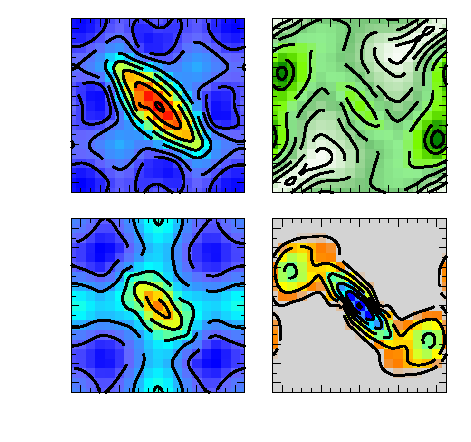
\includegraphics[width={453.00bp},height={453.00bp}]{chapters/results/image/Q0_maps}}%
    \gplfronttext
  \end{picture}%
\endgroup

		\end{column}
		\hfill
		\begin{column}{0.50\textwidth}
			C\textsubscript{2} symmetry
			\begin{itemize}
				\item \textbf{PES}: Several minima
				\item \textbf{Dipole Moment}: Two strong dipole regions
				\item \textbf{VBS}: Dependent on electron donating or withdrawing character of the methoxy groups
				\item \textbf{DBS}: Follows dipole strength
			\end{itemize}
			\vspace{0pt}
			\begin{columns}[b]
				\hfill
				\begin{column}{0.3\textwidth}
					\centering
					\put(-20,5){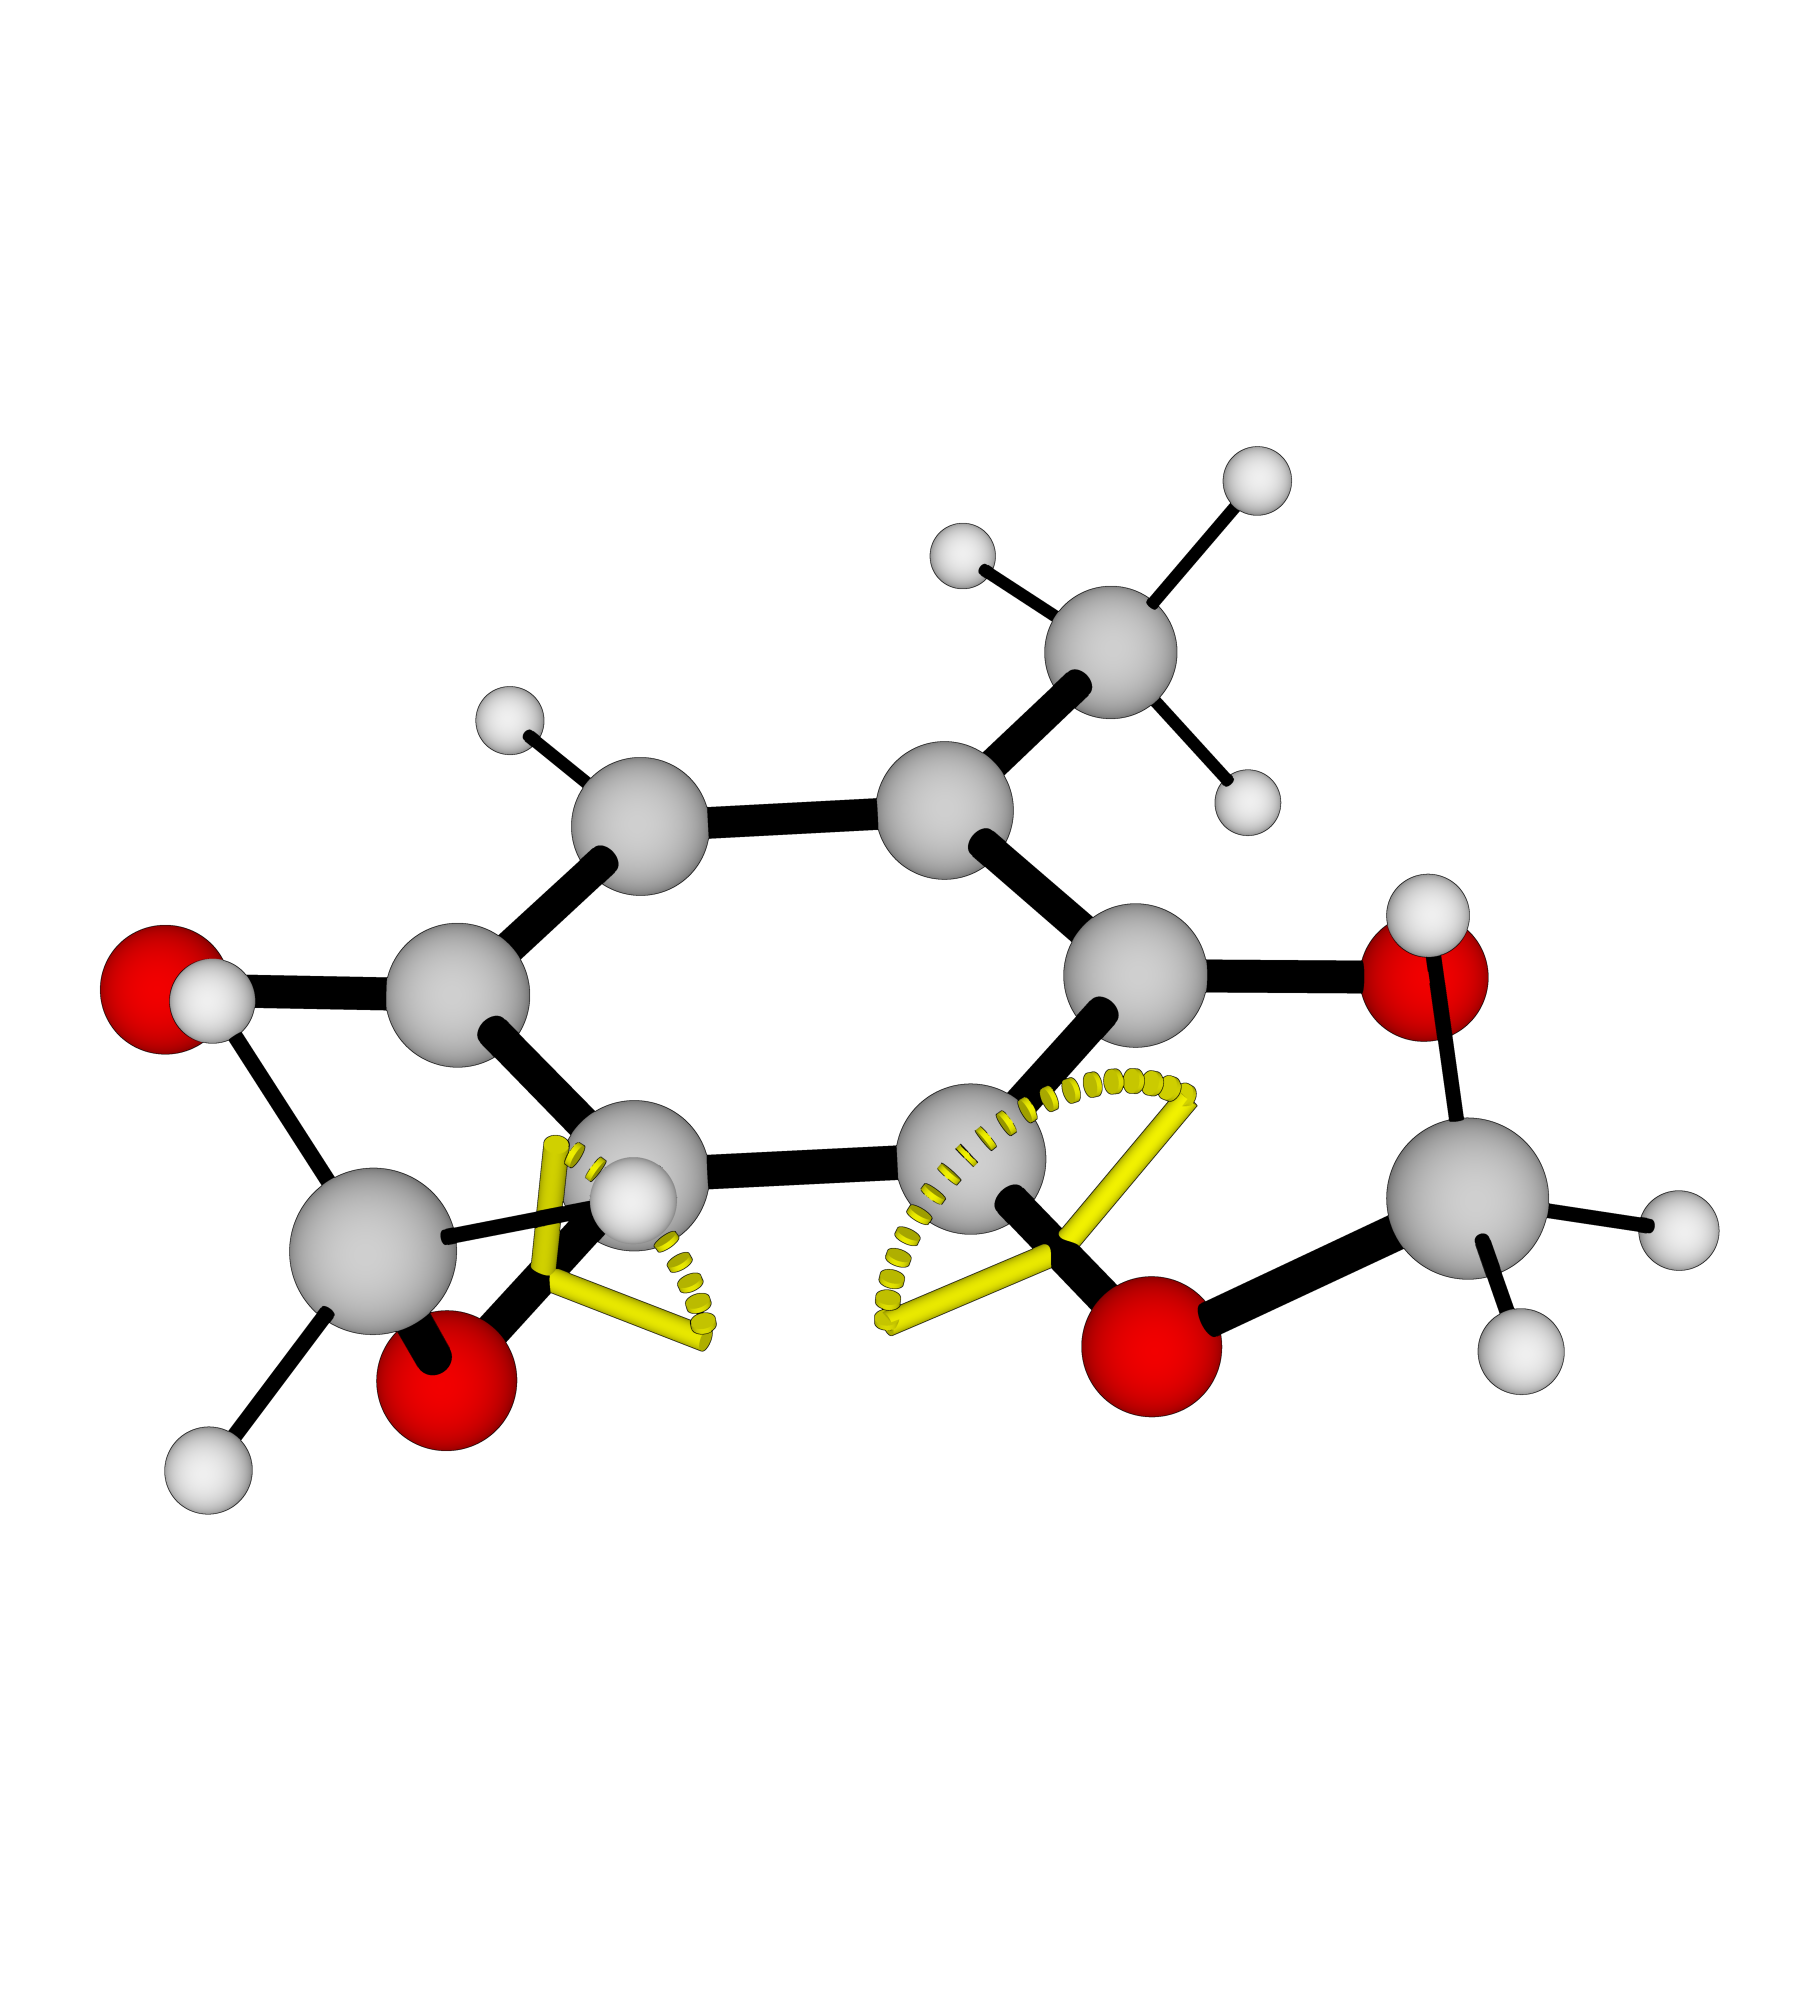
\includegraphics[width=1.3\textwidth]{Figs/dihedrals.png}}
					$\Psi$ and $\Phi$
				\end{column}
				\begin{column}{0.3\textwidth}
					\centering
					\put(-20,10){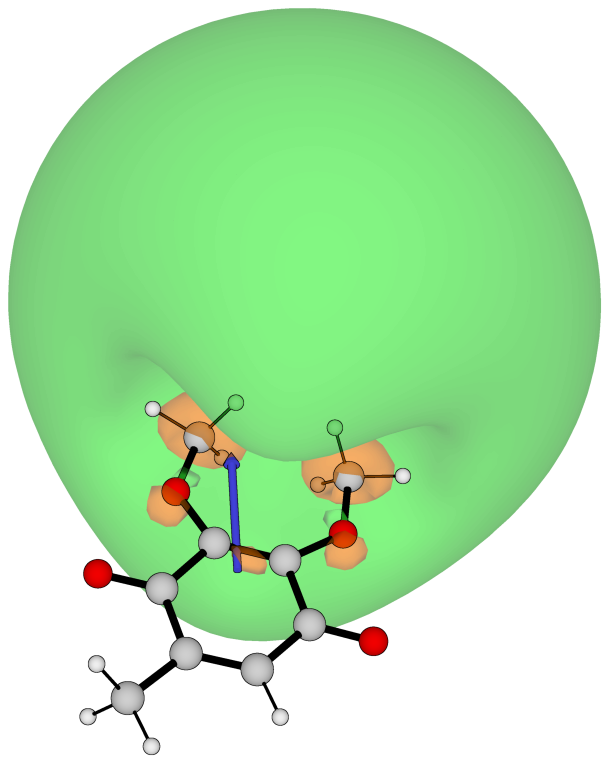
\includegraphics[width=1.0\textwidth]{Figs/Q0_181.png}}
					DBS
				\end{column}
				\begin{column}{0.3\textwidth}
					\centering
					\put(-25,25){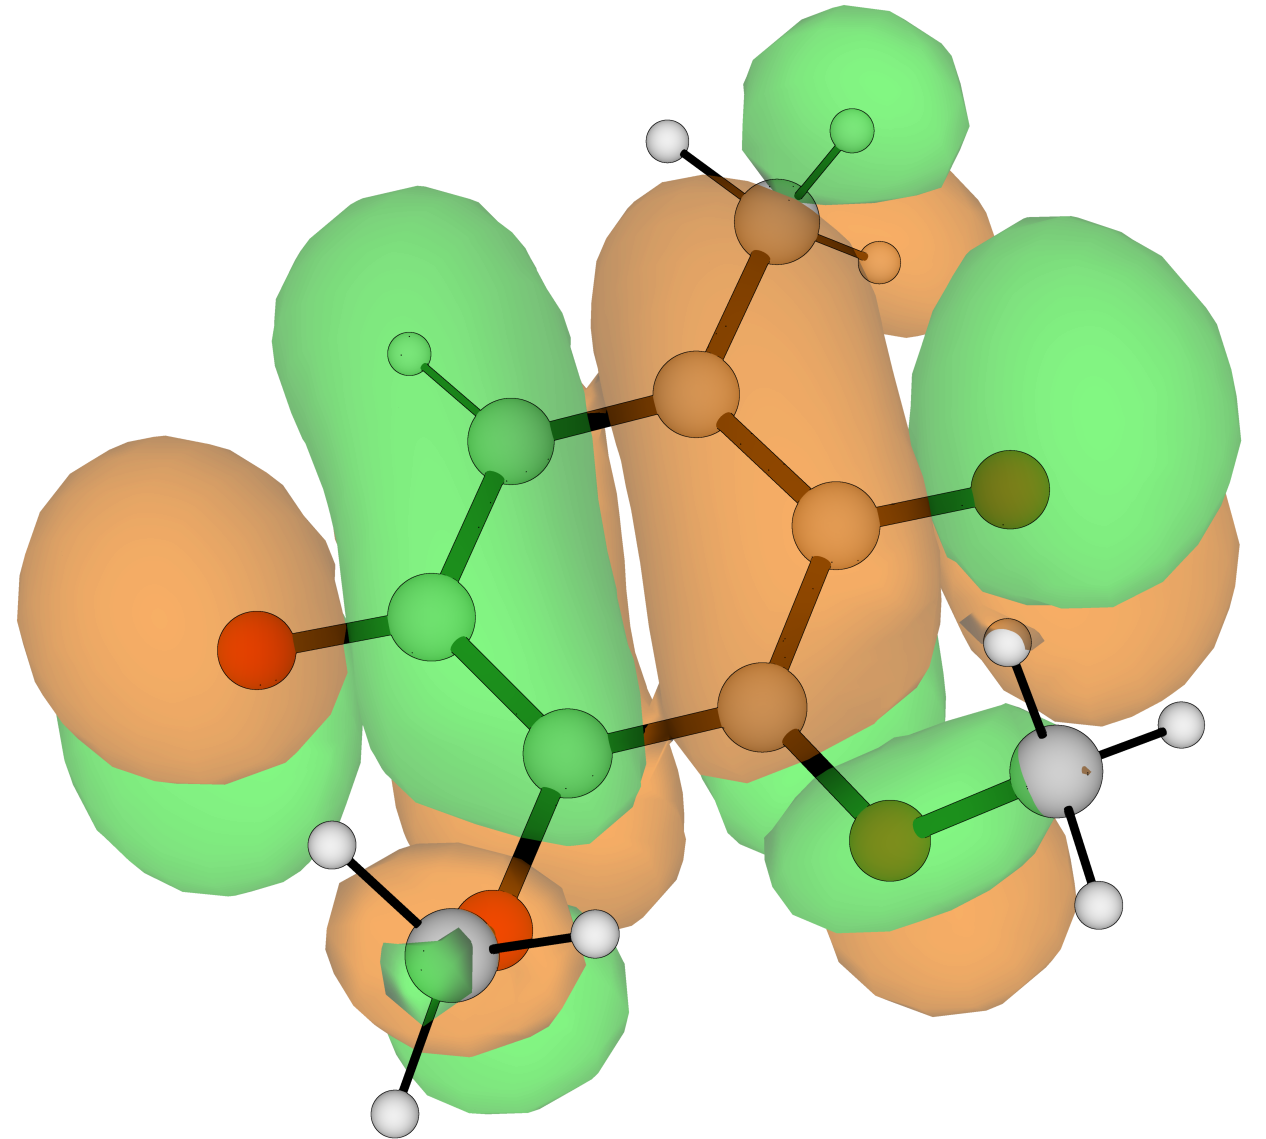
\includegraphics[width=1.0\textwidth]{Figs/Q0_52_VBS.png}}
					VBA
				\end{column}
			\end{columns}
		\end{column}
	\end{columns}
\end{frame}

\begin{frame}{\huge Potential Energy Surfaces of Q1}\large
	\begin{columns}[t]
		\begin{column}{0.4\textwidth}
			\footnotesize
			\vspace{-22pt}
			% GNUPLOT: LaTeX picture with Postscript
\begingroup
  \makeatletter
  \providecommand\color[2][]{%
    \GenericError{(gnuplot) \space\space\space\@spaces}{%
      Package color not loaded in conjunction with
      terminal option `colourtext'%
    }{See the gnuplot documentation for explanation.%
    }{Either use 'blacktext' in gnuplot or load the package
      color.sty in LaTeX.}%
    \renewcommand\color[2][]{}%
  }%
  \providecommand\includegraphics[2][]{%
    \GenericError{(gnuplot) \space\space\space\@spaces}{%
      Package graphicx or graphics not loaded%
    }{See the gnuplot documentation for explanation.%
    }{The gnuplot epslatex terminal needs graphicx.sty or graphics.sty.}%
    \renewcommand\includegraphics[2][]{}%
  }%
  \providecommand\rotatebox[2]{#2}%
  \@ifundefined{ifGPcolor}{%
    \newif\ifGPcolor
    \GPcolortrue
  }{}%
  \@ifundefined{ifGPblacktext}{%
    \newif\ifGPblacktext
    \GPblacktexttrue
  }{}%
  % define a \g@addto@macro without @ in the name:
  \let\gplgaddtomacro\g@addto@macro
  % define empty templates for all commands taking text:
  \gdef\gplbacktext{}%
  \gdef\gplfronttext{}%
  \makeatother
  \ifGPblacktext
    % no textcolor at all
    \def\colorrgb#1{}%
    \def\colorgray#1{}%
  \else
    % gray or color?
    \ifGPcolor
      \def\colorrgb#1{\color[rgb]{#1}}%
      \def\colorgray#1{\color[gray]{#1}}%
      \expandafter\def\csname LTw\endcsname{\color{white}}%
      \expandafter\def\csname LTb\endcsname{\color{black}}%
      \expandafter\def\csname LTa\endcsname{\color{black}}%
      \expandafter\def\csname LT0\endcsname{\color[rgb]{1,0,0}}%
      \expandafter\def\csname LT1\endcsname{\color[rgb]{0,1,0}}%
      \expandafter\def\csname LT2\endcsname{\color[rgb]{0,0,1}}%
      \expandafter\def\csname LT3\endcsname{\color[rgb]{1,0,1}}%
      \expandafter\def\csname LT4\endcsname{\color[rgb]{0,1,1}}%
      \expandafter\def\csname LT5\endcsname{\color[rgb]{1,1,0}}%
      \expandafter\def\csname LT6\endcsname{\color[rgb]{0,0,0}}%
      \expandafter\def\csname LT7\endcsname{\color[rgb]{1,0.3,0}}%
      \expandafter\def\csname LT8\endcsname{\color[rgb]{0.5,0.5,0.5}}%
    \else
      % gray
      \def\colorrgb#1{\color{black}}%
      \def\colorgray#1{\color[gray]{#1}}%
      \expandafter\def\csname LTw\endcsname{\color{white}}%
      \expandafter\def\csname LTb\endcsname{\color{black}}%
      \expandafter\def\csname LTa\endcsname{\color{black}}%
      \expandafter\def\csname LT0\endcsname{\color{black}}%
      \expandafter\def\csname LT1\endcsname{\color{black}}%
      \expandafter\def\csname LT2\endcsname{\color{black}}%
      \expandafter\def\csname LT3\endcsname{\color{black}}%
      \expandafter\def\csname LT4\endcsname{\color{black}}%
      \expandafter\def\csname LT5\endcsname{\color{black}}%
      \expandafter\def\csname LT6\endcsname{\color{black}}%
      \expandafter\def\csname LT7\endcsname{\color{black}}%
      \expandafter\def\csname LT8\endcsname{\color{black}}%
    \fi
  \fi
    \setlength{\unitlength}{0.0500bp}%
    \ifx\gptboxheight\undefined%
      \newlength{\gptboxheight}%
      \newlength{\gptboxwidth}%
      \newsavebox{\gptboxtext}%
    \fi%
    \setlength{\fboxrule}{0.5pt}%
    \setlength{\fboxsep}{1pt}%
    \definecolor{tbcol}{rgb}{1,1,1}%
\begin{picture}(6980.00,6980.00)%
    \gplgaddtomacro\gplbacktext{%
    }%
    \gplgaddtomacro\gplfronttext{%
      \csname LTb\endcsname%%
      \put(389,3994){\makebox(0,0)[r]{\strut{}$-160$}}%
      \csname LTb\endcsname%%
      \put(389,4326){\makebox(0,0)[r]{\strut{}$-120$}}%
      \csname LTb\endcsname%%
      \put(389,4659){\makebox(0,0)[r]{\strut{}$-80$}}%
      \csname LTb\endcsname%%
      \put(389,4991){\makebox(0,0)[r]{\strut{}$-40$}}%
      \csname LTb\endcsname%%
      \put(389,5324){\makebox(0,0)[r]{\strut{}$0$}}%
      \csname LTb\endcsname%%
      \put(389,5656){\makebox(0,0)[r]{\strut{}$40$}}%
      \csname LTb\endcsname%%
      \put(389,5989){\makebox(0,0)[r]{\strut{}$80$}}%
      \csname LTb\endcsname%%
      \put(389,6321){\makebox(0,0)[r]{\strut{}$120$}}%
      \csname LTb\endcsname%%
      \put(389,6654){\makebox(0,0)[r]{\strut{}$160$}}%
      \csname LTb\endcsname%%
      \put(487,3652){\makebox(0,0){\strut{}}}%
      \csname LTb\endcsname%%
      \put(986,3652){\makebox(0,0){\strut{}}}%
      \csname LTb\endcsname%%
      \put(1484,3652){\makebox(0,0){\strut{}}}%
      \csname LTb\endcsname%%
      \put(1983,3652){\makebox(0,0){\strut{}}}%
      \csname LTb\endcsname%%
      \put(2482,3652){\makebox(0,0){\strut{}}}%
      \csname LTb\endcsname%%
      \put(2981,3652){\makebox(0,0){\strut{}}}%
      \csname LTb\endcsname%%
      \put(3480,3652){\makebox(0,0){\strut{}}}%
      \csname LTb\endcsname%%
      \put(32,5324){\rotatebox{-270.00}{\makebox(0,0){\normalsize $\Psi$}}}%
      \csname LTb\endcsname%%
      \put(1669,5498){\rotatebox{-63.00}{\makebox(0,0){\strut{}\textcolor{black}{\footnotesize 500}}}}%
      \csname LTb\endcsname%%
      \put(2272,5409){\rotatebox{130.00}{\makebox(0,0){\strut{}\textcolor{black}{\footnotesize 400}}}}%
      \csname LTb\endcsname%%
      \put(1758,5160){\rotatebox{-46.00}{\makebox(0,0){\strut{}\textcolor{black}{\footnotesize 400}}}}%
      \csname LTb\endcsname%%
      \put(1725,5940){\rotatebox{157.00}{\makebox(0,0){\strut{}\textcolor{black}{\footnotesize 300}}}}%
      \csname LTb\endcsname%%
      \put(1870,4897){\rotatebox{-39.00}{\makebox(0,0){\strut{}\textcolor{black}{\footnotesize 300}}}}%
      \csname LTb\endcsname%%
      \put(2641,5261){\rotatebox{115.00}{\makebox(0,0){\strut{}\textcolor{black}{\footnotesize 200}}}}%
      \csname LTb\endcsname%%
      \put(1191,6171){\rotatebox{-140.00}{\makebox(0,0){\strut{}\textcolor{black}{\footnotesize 200}}}}%
      \csname LTb\endcsname%%
      \put(1989,4683){\rotatebox{-24.00}{\makebox(0,0){\strut{}\textcolor{black}{\footnotesize 200}}}}%
      \csname LTb\endcsname%%
      \put(1191,4995){\rotatebox{39.00}{\makebox(0,0){\strut{}\textcolor{black}{\footnotesize 100}}}}%
      \csname LTb\endcsname%%
      \put(1142,6544){\rotatebox{44.00}{\makebox(0,0){\strut{}\textcolor{black}{\footnotesize 100}}}}%
      \csname LTb\endcsname%%
      \put(2474,6418){\rotatebox{62.00}{\makebox(0,0){\strut{}\textcolor{black}{\footnotesize 100}}}}%
      \csname LTb\endcsname%%
      \put(2748,5336){\rotatebox{-73.00}{\makebox(0,0){\strut{}\textcolor{black}{\footnotesize 100}}}}%
      \csname LTb\endcsname%%
      \put(990,4433){\rotatebox{-33.00}{\makebox(0,0){\strut{}\textcolor{black}{\footnotesize 100}}}}%
      \csname LTb\endcsname%%
      \put(2588,4180){\rotatebox{-44.00}{\makebox(0,0){\strut{}\textcolor{black}{\footnotesize 100}}}}%
      \csname LTb\endcsname%%
      \put(585,5638){\rotatebox{-104.00}{\makebox(0,0){\strut{}\textcolor{black}{\footnotesize 50}}}}%
      \csname LTb\endcsname%%
      \put(1865,6569){\rotatebox{158.00}{\makebox(0,0){\strut{}\textcolor{black}{\footnotesize 50}}}}%
      \csname LTb\endcsname%%
      \put(1541,3978){\rotatebox{-72.00}{\makebox(0,0){\strut{}\textcolor{black}{\footnotesize 50}}}}%
      \csname LTb\endcsname%%
      \put(2926,5567){\rotatebox{-139.00}{\makebox(0,0){\strut{}\textcolor{black}{\footnotesize 50}}}}%
      \csname LTb\endcsname%%
      \put(1983,6943){\makebox(0,0){\strut{}Conformational Energy (meV)}}%
    }%
    \gplgaddtomacro\gplbacktext{%
    }%
    \gplgaddtomacro\gplfronttext{%
      \csname LTb\endcsname%%
      \put(3695,3994){\makebox(0,0)[r]{\strut{}}}%
      \csname LTb\endcsname%%
      \put(3695,4326){\makebox(0,0)[r]{\strut{}}}%
      \csname LTb\endcsname%%
      \put(3695,4659){\makebox(0,0)[r]{\strut{}}}%
      \csname LTb\endcsname%%
      \put(3695,4991){\makebox(0,0)[r]{\strut{}}}%
      \csname LTb\endcsname%%
      \put(3695,5324){\makebox(0,0)[r]{\strut{}}}%
      \csname LTb\endcsname%%
      \put(3695,5656){\makebox(0,0)[r]{\strut{}}}%
      \csname LTb\endcsname%%
      \put(3695,5989){\makebox(0,0)[r]{\strut{}}}%
      \csname LTb\endcsname%%
      \put(3695,6321){\makebox(0,0)[r]{\strut{}}}%
      \csname LTb\endcsname%%
      \put(3695,6654){\makebox(0,0)[r]{\strut{}}}%
      \csname LTb\endcsname%%
      \put(3793,3652){\makebox(0,0){\strut{}}}%
      \csname LTb\endcsname%%
      \put(4291,3652){\makebox(0,0){\strut{}}}%
      \csname LTb\endcsname%%
      \put(4790,3652){\makebox(0,0){\strut{}}}%
      \csname LTb\endcsname%%
      \put(5289,3652){\makebox(0,0){\strut{}}}%
      \csname LTb\endcsname%%
      \put(5788,3652){\makebox(0,0){\strut{}}}%
      \csname LTb\endcsname%%
      \put(6287,3652){\makebox(0,0){\strut{}}}%
      \csname LTb\endcsname%%
      \put(6785,3652){\makebox(0,0){\strut{}}}%
      \csname LTb\endcsname%%
      \put(5700,4218){\rotatebox{43.00}{\makebox(0,0){\strut{}\textcolor{black}{\footnotesize 3.0}}}}%
      \csname LTb\endcsname%%
      \put(5522,5222){\rotatebox{129.00}{\makebox(0,0){\strut{}\textcolor{black}{\footnotesize 2.5}}}}%
      \csname LTb\endcsname%%
      \put(4353,6459){\rotatebox{-72.00}{\makebox(0,0){\strut{}\textcolor{black}{\footnotesize 2.5}}}}%
      \csname LTb\endcsname%%
      \put(5372,6661){\makebox(0,0){\strut{}\textcolor{black}{\footnotesize 2.5}}}%
      \csname LTb\endcsname%%
      \put(4515,3989){\rotatebox{40.00}{\makebox(0,0){\strut{}\textcolor{black}{\footnotesize 2.5}}}}%
      \csname LTb\endcsname%%
      \put(5552,4386){\rotatebox{42.00}{\makebox(0,0){\strut{}\textcolor{black}{\footnotesize 2.5}}}}%
      \csname LTb\endcsname%%
      \put(6545,4794){\rotatebox{-22.00}{\makebox(0,0){\strut{}\textcolor{black}{\footnotesize 2.5}}}}%
      \csname LTb\endcsname%%
      \put(4187,6670){\rotatebox{-108.00}{\makebox(0,0){\strut{}\textcolor{black}{\footnotesize 2.0}}}}%
      \csname LTb\endcsname%%
      \put(4560,6009){\rotatebox{-4.00}{\makebox(0,0){\strut{}\textcolor{black}{\footnotesize 2.0}}}}%
      \csname LTb\endcsname%%
      \put(5567,6455){\rotatebox{-5.00}{\makebox(0,0){\strut{}\textcolor{black}{\footnotesize 2.0}}}}%
      \csname LTb\endcsname%%
      \put(5101,4265){\rotatebox{24.00}{\makebox(0,0){\strut{}\textcolor{black}{\footnotesize 2.0}}}}%
      \csname LTb\endcsname%%
      \put(5251,5011){\rotatebox{145.00}{\makebox(0,0){\strut{}\textcolor{black}{\footnotesize 2.0}}}}%
      \csname LTb\endcsname%%
      \put(5086,5696){\rotatebox{-23.00}{\makebox(0,0){\strut{}\textcolor{black}{\footnotesize 2.0}}}}%
      \csname LTb\endcsname%%
      \put(5973,5109){\rotatebox{-19.00}{\makebox(0,0){\strut{}\textcolor{black}{\footnotesize 2.0}}}}%
      \csname LTb\endcsname%%
      \put(4006,5346){\rotatebox{50.00}{\makebox(0,0){\strut{}\textcolor{black}{\footnotesize 1.5}}}}%
      \csname LTb\endcsname%%
      \put(4845,5166){\rotatebox{-50.00}{\makebox(0,0){\strut{}\textcolor{black}{\footnotesize 1.5}}}}%
      \csname LTb\endcsname%%
      \put(4906,4402){\rotatebox{-173.00}{\makebox(0,0){\strut{}\textcolor{black}{\footnotesize 1.5}}}}%
      \csname LTb\endcsname%%
      \put(6065,6324){\rotatebox{-155.00}{\makebox(0,0){\strut{}\textcolor{black}{\footnotesize 1.5}}}}%
      \csname LTb\endcsname%%
      \put(5236,5857){\rotatebox{-36.00}{\makebox(0,0){\strut{}\textcolor{black}{\footnotesize 1.5}}}}%
      \csname LTb\endcsname%%
      \put(6199,5401){\rotatebox{16.00}{\makebox(0,0){\strut{}\textcolor{black}{\footnotesize 1.5}}}}%
      \csname LTb\endcsname%%
      \put(3907,4143){\rotatebox{75.00}{\makebox(0,0){\strut{}\textcolor{black}{\footnotesize 1.0}}}}%
      \csname LTb\endcsname%%
      \put(4274,5214){\rotatebox{14.00}{\makebox(0,0){\strut{}\textcolor{black}{\footnotesize 1.0}}}}%
      \csname LTb\endcsname%%
      \put(4620,4529){\rotatebox{-156.00}{\makebox(0,0){\strut{}\textcolor{black}{\footnotesize 1.0}}}}%
      \csname LTb\endcsname%%
      \put(6003,6130){\rotatebox{-158.00}{\makebox(0,0){\strut{}\textcolor{black}{\footnotesize 1.0}}}}%
      \csname LTb\endcsname%%
      \put(6214,5602){\rotatebox{11.00}{\makebox(0,0){\strut{}\textcolor{black}{\footnotesize 1.0}}}}%
      \csname LTb\endcsname%%
      \put(4533,4880){\rotatebox{116.00}{\makebox(0,0){\strut{}\textcolor{black}{\footnotesize 0.5}}}}%
      \csname LTb\endcsname%%
      \put(5289,6943){\makebox(0,0){Dipole Strength (Debye)}}%
    }%
    \gplgaddtomacro\gplbacktext{%
    }%
    \gplgaddtomacro\gplfronttext{%
      \csname LTb\endcsname%%
      \put(389,723){\makebox(0,0)[r]{\strut{}$-160$}}%
      \csname LTb\endcsname%%
      \put(389,1055){\makebox(0,0)[r]{\strut{}$-120$}}%
      \csname LTb\endcsname%%
      \put(389,1388){\makebox(0,0)[r]{\strut{}$-80$}}%
      \csname LTb\endcsname%%
      \put(389,1720){\makebox(0,0)[r]{\strut{}$-40$}}%
      \csname LTb\endcsname%%
      \put(389,2053){\makebox(0,0)[r]{\strut{}$0$}}%
      \csname LTb\endcsname%%
      \put(389,2385){\makebox(0,0)[r]{\strut{}$40$}}%
      \csname LTb\endcsname%%
      \put(389,2718){\makebox(0,0)[r]{\strut{}$80$}}%
      \csname LTb\endcsname%%
      \put(389,3050){\makebox(0,0)[r]{\strut{}$120$}}%
      \csname LTb\endcsname%%
      \put(389,3383){\makebox(0,0)[r]{\strut{}$160$}}%
      \csname LTb\endcsname%%
      \put(487,380){\makebox(0,0){\strut{}$-180$}}%
      \csname LTb\endcsname%%
      \put(986,380){\makebox(0,0){\strut{}$-120$}}%
      \csname LTb\endcsname%%
      \put(1484,380){\makebox(0,0){\strut{}$-60$}}%
      \csname LTb\endcsname%%
      \put(1983,380){\makebox(0,0){\strut{}$0$}}%
      \csname LTb\endcsname%%
      \put(2482,380){\makebox(0,0){\strut{}$60$}}%
      \csname LTb\endcsname%%
      \put(2981,380){\makebox(0,0){\strut{}$120$}}%
      \csname LTb\endcsname%%
      \put(3479,380){\makebox(0,0){\strut{}$180$}}%
      \csname LTb\endcsname%%
      \put(32,2053){\rotatebox{-270.00}{\makebox(0,0){\normalsize $\Psi$}}}%
      \csname LTb\endcsname%%
      \put(1983,117){\makebox(0,0){\normalsize $\Phi$}}%
      \csname LTb\endcsname%%
      \put(1881,2279){\rotatebox{148.00}{\makebox(0,0){\strut{}\textcolor{black}{\footnotesize 1.3}}}}%
      \csname LTb\endcsname%%
      \put(1696,1928){\rotatebox{-45.00}{\makebox(0,0){\strut{}\textcolor{black}{\footnotesize 1.4}}}}%
      \csname LTb\endcsname%%
      \put(2297,2279){\rotatebox{143.00}{\makebox(0,0){\strut{}\textcolor{black}{\footnotesize 1.5}}}}%
      \csname LTb\endcsname%%
      \put(1947,1554){\rotatebox{-45.00}{\makebox(0,0){\strut{}\textcolor{black}{\footnotesize 1.5}}}}%
      \csname LTb\endcsname%%
      \put(1582,2824){\rotatebox{45.00}{\makebox(0,0){\strut{}\textcolor{black}{\footnotesize 1.6}}}}%
      \csname LTb\endcsname%%
      \put(2693,1629){\rotatebox{48.00}{\makebox(0,0){\strut{}\textcolor{black}{\footnotesize 1.6}}}}%
      \csname LTb\endcsname%%
      \put(883,2824){\rotatebox{-34.00}{\makebox(0,0){\strut{}\textcolor{black}{\footnotesize 1.7}}}}%
      \csname LTb\endcsname%%
      \put(1411,1040){\rotatebox{112.00}{\makebox(0,0){\strut{}\textcolor{black}{\footnotesize 1.7}}}}%
      \csname LTb\endcsname%%
      \put(2845,3372){\rotatebox{-135.00}{\makebox(0,0){\strut{}\textcolor{black}{\footnotesize 1.7}}}}%
      \csname LTb\endcsname%%
      \put(2754,783){\rotatebox{-25.00}{\makebox(0,0){\strut{}\textcolor{black}{\footnotesize 1.7}}}}%
      \csname LTb\endcsname%%
      \put(1983,3672){\makebox(0,0){VBA EA (eV)}}%
    }%
    \gplgaddtomacro\gplbacktext{%
    }%
    \gplgaddtomacro\gplfronttext{%
      \csname LTb\endcsname%%
      \put(3695,723){\makebox(0,0)[r]{\strut{}}}%
      \csname LTb\endcsname%%
      \put(3695,1055){\makebox(0,0)[r]{\strut{}}}%
      \csname LTb\endcsname%%
      \put(3695,1388){\makebox(0,0)[r]{\strut{}}}%
      \csname LTb\endcsname%%
      \put(3695,1720){\makebox(0,0)[r]{\strut{}}}%
      \csname LTb\endcsname%%
      \put(3695,2053){\makebox(0,0)[r]{\strut{}}}%
      \csname LTb\endcsname%%
      \put(3695,2385){\makebox(0,0)[r]{\strut{}}}%
      \csname LTb\endcsname%%
      \put(3695,2718){\makebox(0,0)[r]{\strut{}}}%
      \csname LTb\endcsname%%
      \put(3695,3050){\makebox(0,0)[r]{\strut{}}}%
      \csname LTb\endcsname%%
      \put(3695,3383){\makebox(0,0)[r]{\strut{}}}%
      \csname LTb\endcsname%%
      \put(3793,380){\makebox(0,0){\strut{}$-180$}}%
      \csname LTb\endcsname%%
      \put(4291,380){\makebox(0,0){\strut{}$-120$}}%
      \csname LTb\endcsname%%
      \put(4790,380){\makebox(0,0){\strut{}$-60$}}%
      \csname LTb\endcsname%%
      \put(5289,380){\makebox(0,0){\strut{}$0$}}%
      \csname LTb\endcsname%%
      \put(5788,380){\makebox(0,0){\strut{}$60$}}%
      \csname LTb\endcsname%%
      \put(6287,380){\makebox(0,0){\strut{}$120$}}%
      \csname LTb\endcsname%%
      \put(6785,380){\makebox(0,0){\strut{}$180$}}%
      \csname LTb\endcsname%%
      \put(5289,117){\makebox(0,0){\normalsize $\Phi$}}%
      \csname LTb\endcsname%%
      \put(5528,1735){\rotatebox{-34.00}{\makebox(0,0){\strut{}\textcolor{black}{\footnotesize 9}}}}%
      \csname LTb\endcsname%%
      \put(5878,726){\rotatebox{-22.00}{\makebox(0,0){\strut{}\textcolor{black}{\footnotesize 9}}}}%
      \csname LTb\endcsname%%
      \put(5637,1104){\rotatebox{69.00}{\makebox(0,0){\strut{}\textcolor{black}{\footnotesize 6}}}}%
      \csname LTb\endcsname%%
      \put(5502,2068){\rotatebox{-38.00}{\makebox(0,0){\strut{}\textcolor{black}{\footnotesize 6}}}}%
      \csname LTb\endcsname%%
      \put(6181,648){\rotatebox{-151.00}{\makebox(0,0){\strut{}\textcolor{black}{\footnotesize 6}}}}%
      \csname LTb\endcsname%%
      \put(4831,3035){\rotatebox{39.00}{\makebox(0,0){\strut{}\textcolor{black}{\footnotesize 3}}}}%
      \csname LTb\endcsname%%
      \put(5576,1294){\rotatebox{70.00}{\makebox(0,0){\strut{}\textcolor{black}{\footnotesize 3}}}}%
      \csname LTb\endcsname%%
      \put(5516,2146){\rotatebox{-39.00}{\makebox(0,0){\strut{}\textcolor{black}{\footnotesize 3}}}}%
      \csname LTb\endcsname%%
      \put(6392,679){\rotatebox{-131.00}{\makebox(0,0){\strut{}\textcolor{black}{\footnotesize 3}}}}%
      \csname LTb\endcsname%%
      \put(6108,3458){\rotatebox{24.00}{\makebox(0,0){\strut{}\textcolor{black}{\footnotesize 3}}}}%
      \csname LTb\endcsname%%
      \put(5126,3337){\rotatebox{91.00}{\makebox(0,0){\strut{}\textcolor{black}{\footnotesize 1}}}}%
      \csname LTb\endcsname%%
      \put(6211,3433){\rotatebox{28.00}{\makebox(0,0){\strut{}\textcolor{black}{\footnotesize 1}}}}%
      \csname LTb\endcsname%%
      \put(5332,1584){\rotatebox{128.00}{\makebox(0,0){\strut{}\textcolor{black}{\footnotesize 1}}}}%
      \csname LTb\endcsname%%
      \put(5592,2159){\rotatebox{-34.00}{\makebox(0,0){\strut{}\textcolor{black}{\footnotesize 1}}}}%
      \csname LTb\endcsname%%
      \put(6497,707){\rotatebox{-116.00}{\makebox(0,0){\strut{}\textcolor{black}{\footnotesize 1}}}}%
      \csname LTb\endcsname%%
      \put(4242,2502){\makebox(0,0){\strut{}\textcolor{black}{\normalsize \textbf{C}}}}%
      \csname LTb\endcsname%%
      \put(6336,1963){\makebox(0,0){\strut{}\textcolor{black}{\normalsize \textbf{B}}}}%
      \csname LTb\endcsname%%
      \put(4930,1753){\makebox(0,0){\strut{}\textcolor{black}{\normalsize \textbf{A}}}}%
      \csname LTb\endcsname%%
      \put(5289,3672){\makebox(0,0){DBA EA (meV)}}%
    }%
    \gplbacktext
    \put(0,0){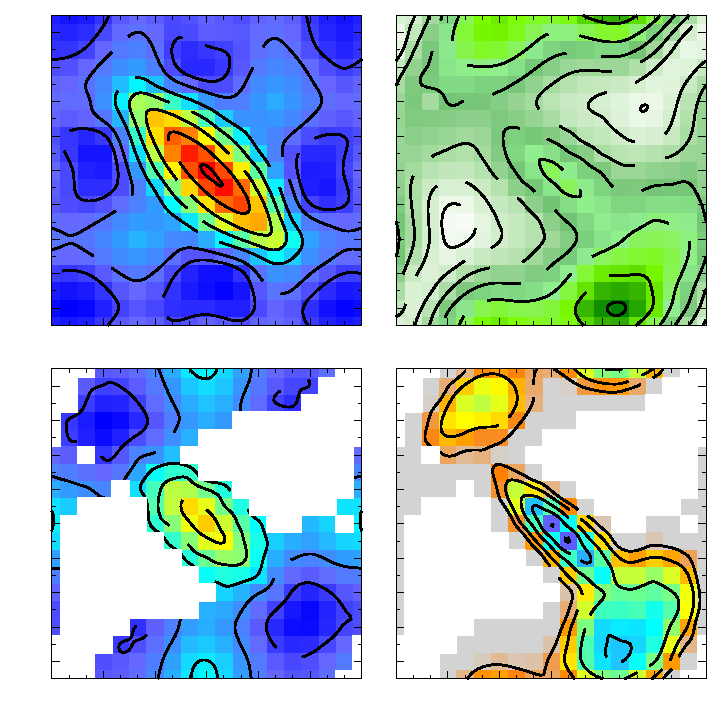
\includegraphics[width={349.00bp},height={349.00bp}]{Q1_maps}}%
    \gplfronttext
  \end{picture}%
\endgroup

		\end{column}
		\hfill
		\begin{column}{0.50\textwidth}
			  Similar to Q0, though isoprene tail breaks the symmetry.
			\begin{itemize}
				\item \textbf{PES}: Isoprene tail distant, analogous to Q0.
				\item \textbf{Dipole Moment}: Isoprene adds fixed dipole. 
				\item \textbf{VBS}: Isoprene tail has minor effect. 
				\item \textbf{DBS}: Isoprene has a pronounced effect.
			\end{itemize}
			\vspace{8pt}
			\begin{columns}[b]
				\hfill
				\begin{column}{0.3\textwidth}
					\centering 
					\put(-35,10){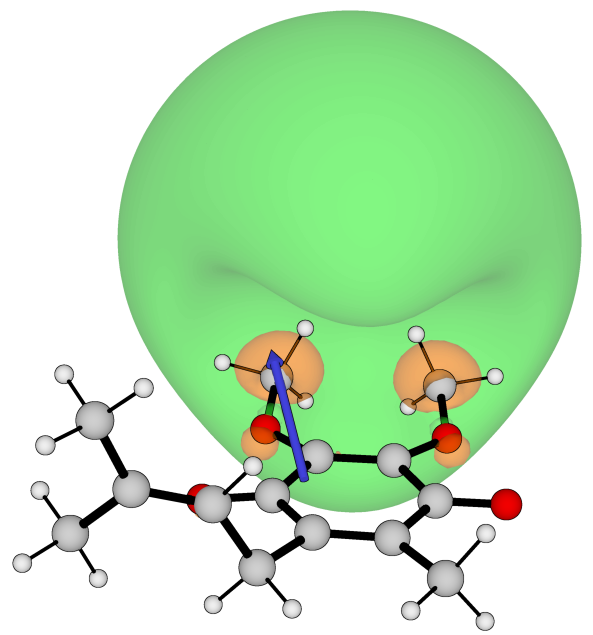
\includegraphics[width=1.2\textwidth]{Figs/Q1_199.png}}
					\textbf{A}
				\end{column}
				\begin{column}{0.3\textwidth}
					\centering
					\put(-30,10){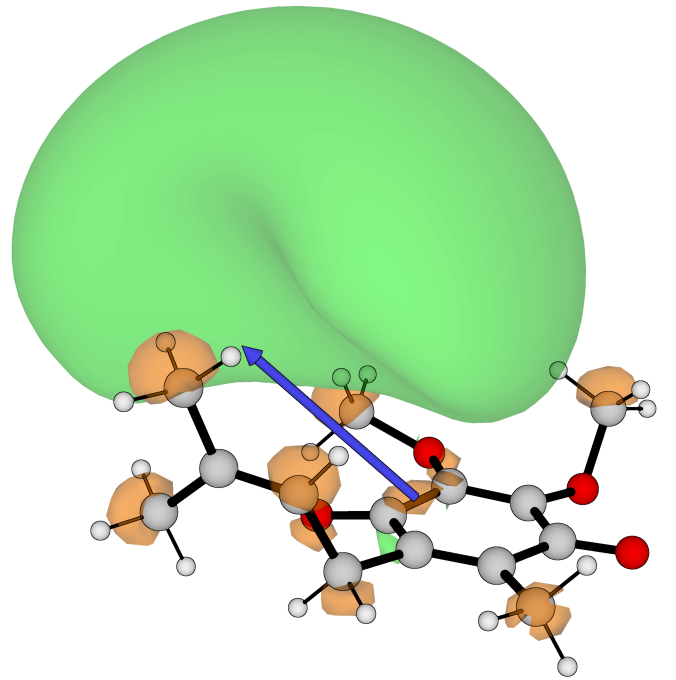
\includegraphics[width=1.2\textwidth]{Figs/Q1_249.png}}
					\textbf{B}
				\end{column}
				\begin{column}{0.3\textwidth}
					\centering 
					\put(-30,5){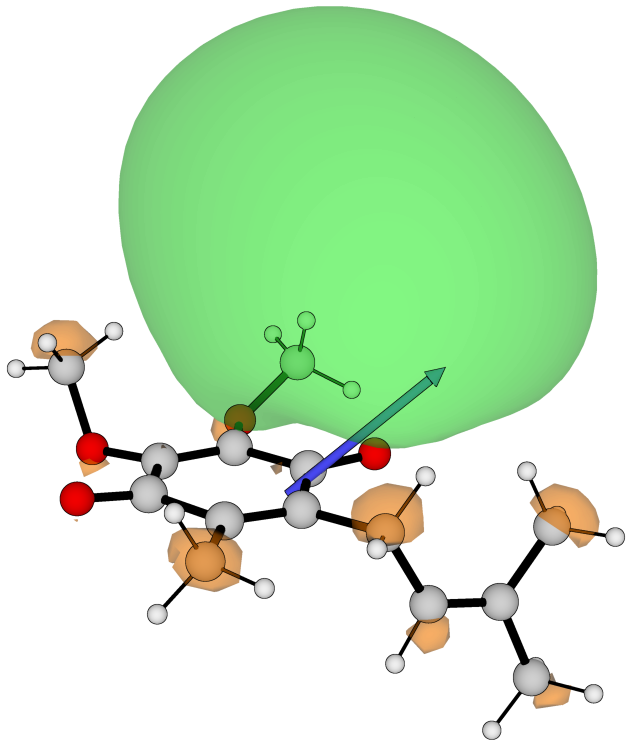
\includegraphics[width=1.2\textwidth]{Figs/Q1_112.png}}
					\textbf{C}
				\end{column}
			\end{columns}
		\end{column}
	\end{columns}
\end{frame}

\begin{frame}
	\frametitle{\huge DBS Populations}\large
	Distinct populations of dipole-bound anions (DBS) are observed\\
	\begin{itemize}
		\item Different regions correlate differently to the dipole strength
		\item \textbf{Region A}: Nearly linear relationship between binding energy and dipole strength
		\item \textbf{Regions B \& C}: Less pronounced correlation. DBS closer to $\pi$ system
	\end{itemize}
	\vspace{5pt}
	\begin{columns}[c]
		\begin{column}{0.62\textwidth}
			\centering
			\small	
			% GNUPLOT: LaTeX picture with Postscript
\begingroup
  \makeatletter
  \providecommand\color[2][]{%
    \GenericError{(gnuplot) \space\space\space\@spaces}{%
      Package color not loaded in conjunction with
      terminal option `colourtext'%
    }{See the gnuplot documentation for explanation.%
    }{Either use 'blacktext' in gnuplot or load the package
      color.sty in LaTeX.}%
    \renewcommand\color[2][]{}%
  }%
  \providecommand\includegraphics[2][]{%
    \GenericError{(gnuplot) \space\space\space\@spaces}{%
      Package graphicx or graphics not loaded%
    }{See the gnuplot documentation for explanation.%
    }{The gnuplot epslatex terminal needs graphicx.sty or graphics.sty.}%
    \renewcommand\includegraphics[2][]{}%
  }%
  \providecommand\rotatebox[2]{#2}%
  \@ifundefined{ifGPcolor}{%
    \newif\ifGPcolor
    \GPcolortrue
  }{}%
  \@ifundefined{ifGPblacktext}{%
    \newif\ifGPblacktext
    \GPblacktexttrue
  }{}%
  % define a \g@addto@macro without @ in the name:
  \let\gplgaddtomacro\g@addto@macro
  % define empty templates for all commands taking text:
  \gdef\gplbacktext{}%
  \gdef\gplfronttext{}%
  \makeatother
  \ifGPblacktext
    % no textcolor at all
    \def\colorrgb#1{}%
    \def\colorgray#1{}%
  \else
    % gray or color?
    \ifGPcolor
      \def\colorrgb#1{\color[rgb]{#1}}%
      \def\colorgray#1{\color[gray]{#1}}%
      \expandafter\def\csname LTw\endcsname{\color{white}}%
      \expandafter\def\csname LTb\endcsname{\color{black}}%
      \expandafter\def\csname LTa\endcsname{\color{black}}%
      \expandafter\def\csname LT0\endcsname{\color[rgb]{1,0,0}}%
      \expandafter\def\csname LT1\endcsname{\color[rgb]{0,1,0}}%
      \expandafter\def\csname LT2\endcsname{\color[rgb]{0,0,1}}%
      \expandafter\def\csname LT3\endcsname{\color[rgb]{1,0,1}}%
      \expandafter\def\csname LT4\endcsname{\color[rgb]{0,1,1}}%
      \expandafter\def\csname LT5\endcsname{\color[rgb]{1,1,0}}%
      \expandafter\def\csname LT6\endcsname{\color[rgb]{0,0,0}}%
      \expandafter\def\csname LT7\endcsname{\color[rgb]{1,0.3,0}}%
      \expandafter\def\csname LT8\endcsname{\color[rgb]{0.5,0.5,0.5}}%
    \else
      % gray
      \def\colorrgb#1{\color{black}}%
      \def\colorgray#1{\color[gray]{#1}}%
      \expandafter\def\csname LTw\endcsname{\color{white}}%
      \expandafter\def\csname LTb\endcsname{\color{black}}%
      \expandafter\def\csname LTa\endcsname{\color{black}}%
      \expandafter\def\csname LT0\endcsname{\color{black}}%
      \expandafter\def\csname LT1\endcsname{\color{black}}%
      \expandafter\def\csname LT2\endcsname{\color{black}}%
      \expandafter\def\csname LT3\endcsname{\color{black}}%
      \expandafter\def\csname LT4\endcsname{\color{black}}%
      \expandafter\def\csname LT5\endcsname{\color{black}}%
      \expandafter\def\csname LT6\endcsname{\color{black}}%
      \expandafter\def\csname LT7\endcsname{\color{black}}%
      \expandafter\def\csname LT8\endcsname{\color{black}}%
    \fi
  \fi
    \setlength{\unitlength}{0.0500bp}%
    \ifx\gptboxheight\undefined%
      \newlength{\gptboxheight}%
      \newlength{\gptboxwidth}%
      \newsavebox{\gptboxtext}%
    \fi%
    \setlength{\fboxrule}{0.5pt}%
    \setlength{\fboxsep}{1pt}%
    \definecolor{tbcol}{rgb}{1,1,1}%
\begin{picture}(6500.00,2540.00)%
    \gplgaddtomacro\gplbacktext{%
      \csname LTb\endcsname%%
      \put(420,453){\makebox(0,0)[r]{\strut{}$0$}}%
      \csname LTb\endcsname%%
      \put(420,729){\makebox(0,0)[r]{\strut{}$2$}}%
      \csname LTb\endcsname%%
      \put(420,1004){\makebox(0,0)[r]{\strut{}$4$}}%
      \csname LTb\endcsname%%
      \put(420,1280){\makebox(0,0)[r]{\strut{}$6$}}%
      \csname LTb\endcsname%%
      \put(420,1555){\makebox(0,0)[r]{\strut{}$8$}}%
      \csname LTb\endcsname%%
      \put(420,1831){\makebox(0,0)[r]{\strut{}$10$}}%
      \csname LTb\endcsname%%
      \put(420,2106){\makebox(0,0)[r]{\strut{}$12$}}%
      \csname LTb\endcsname%%
      \put(420,2382){\makebox(0,0)[r]{\strut{}$14$}}%
      \csname LTb\endcsname%%
      \put(518,277){\makebox(0,0){\strut{}$1.5$}}%
      \csname LTb\endcsname%%
      \put(1181,277){\makebox(0,0){\strut{}$2$}}%
      \csname LTb\endcsname%%
      \put(1843,277){\makebox(0,0){\strut{}$2.5$}}%
      \csname LTb\endcsname%%
      \put(2506,277){\makebox(0,0){\strut{}$3$}}%
      \csname LTb\endcsname%%
      \put(3169,277){\makebox(0,0){\strut{}$3.5$}}%
      \csname LTb\endcsname%%
      \put(810,2354){\makebox(0,0){\strut{}Q0}}%
    }%
    \gplgaddtomacro\gplfronttext{%
      \csname LTb\endcsname%%
      \put(2913,2297){\makebox(0,0)[r]{\strut{}Region A}}%
      \csname LTb\endcsname%%
      \put(2913,2122){\makebox(0,0)[r]{\strut{}Region B}}%
      \csname LTb\endcsname%%
      \put(63,1486){\rotatebox{-270.00}{\makebox(0,0){\strut{}DBS Binding Energy (meV)}}}%
      \csname LTb\endcsname%%
      \put(1976,13){\makebox(0,0){\strut{}Dipole Strength (Debye)}}%
    }%
    \gplgaddtomacro\gplbacktext{%
      \csname LTb\endcsname%%
      \put(3466,453){\makebox(0,0)[r]{\strut{}}}%
      \csname LTb\endcsname%%
      \put(3466,729){\makebox(0,0)[r]{\strut{}}}%
      \csname LTb\endcsname%%
      \put(3466,1004){\makebox(0,0)[r]{\strut{}}}%
      \csname LTb\endcsname%%
      \put(3466,1280){\makebox(0,0)[r]{\strut{}}}%
      \csname LTb\endcsname%%
      \put(3466,1555){\makebox(0,0)[r]{\strut{}}}%
      \csname LTb\endcsname%%
      \put(3466,1831){\makebox(0,0)[r]{\strut{}}}%
      \csname LTb\endcsname%%
      \put(3466,2106){\makebox(0,0)[r]{\strut{}}}%
      \csname LTb\endcsname%%
      \put(3466,2382){\makebox(0,0)[r]{\strut{}}}%
      \csname LTb\endcsname%%
      \put(3564,277){\makebox(0,0){\strut{}$1.5$}}%
      \csname LTb\endcsname%%
      \put(4226,277){\makebox(0,0){\strut{}$2$}}%
      \csname LTb\endcsname%%
      \put(4889,277){\makebox(0,0){\strut{}$2.5$}}%
      \csname LTb\endcsname%%
      \put(5552,277){\makebox(0,0){\strut{}$3$}}%
      \csname LTb\endcsname%%
      \put(6214,277){\makebox(0,0){\strut{}$3.5$}}%
      \csname LTb\endcsname%%
      \put(3855,2354){\makebox(0,0){\strut{}Q1}}%
    }%
    \gplgaddtomacro\gplfronttext{%
      \csname LTb\endcsname%%
      \put(5959,2385){\makebox(0,0)[r]{\strut{}Region A}}%
      \csname LTb\endcsname%%
      \put(5959,2209){\makebox(0,0)[r]{\strut{}Region B}}%
      \csname LTb\endcsname%%
      \put(5959,2034){\makebox(0,0)[r]{\strut{}Region C}}%
      \csname LTb\endcsname%%
      \put(5021,13){\makebox(0,0){\strut{}Dipole Strength (Debye)}}%
    }%
    \gplbacktext
    \put(0,0){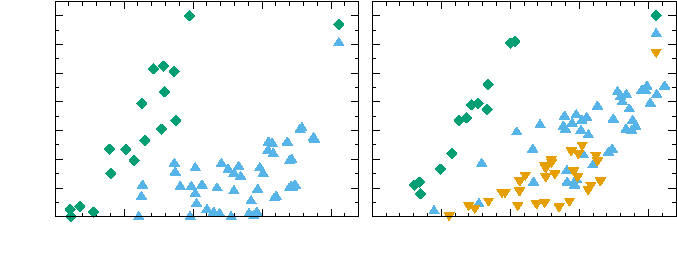
\includegraphics[width={325.00bp},height={127.00bp}]{Figs/DvsDBS}}%
    \gplfronttext
  \end{picture}%
\endgroup

		\end{column}
		\hspace{30pt}
		\begin{column}{0.3\textwidth}
			\centering
	 		\textbf{A} 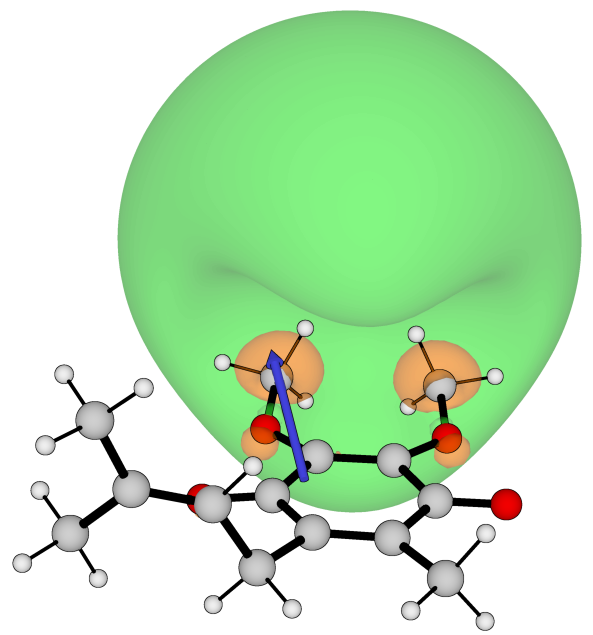
\includegraphics[width=0.41\textwidth]{Figs/Q1_199.png} \hfill\\
			\textbf{B} 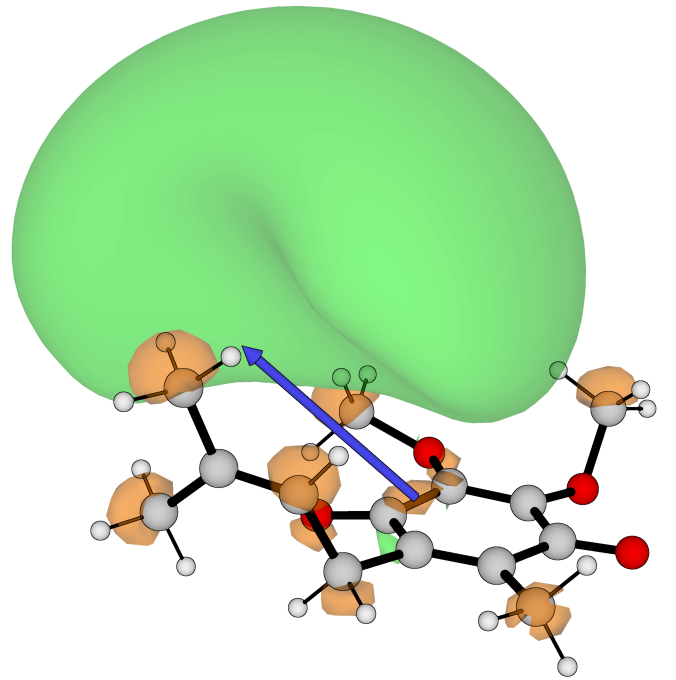
\includegraphics[width=0.41\textwidth]{Figs/Q1_249.png} \hfill
			\textbf{C} 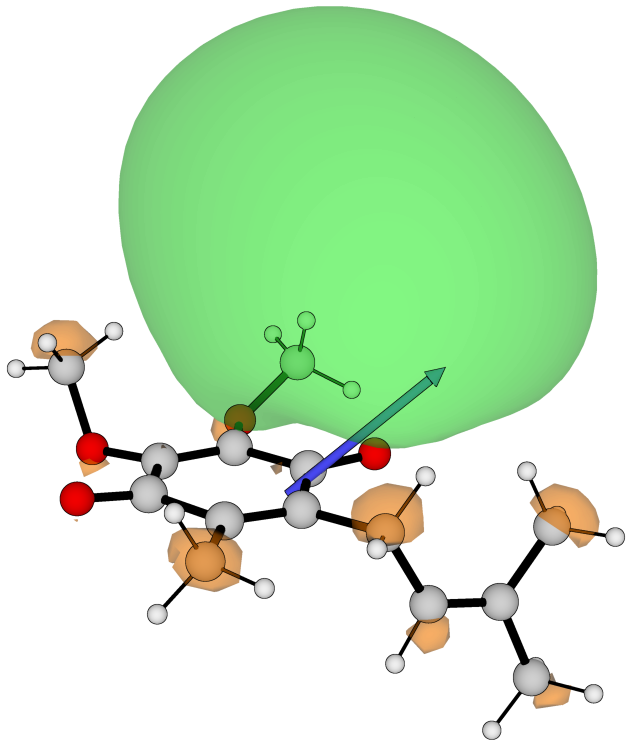
\includegraphics[width=0.41\textwidth]{Figs/Q1_112.png} \hfill 
		\end{column}
	\end{columns}		
\end{frame}

\begin{frame}
	\frametitle{\huge Interaction with solvent molecules (DBS)}\large
	%A directed interaction with small molecules strongly stabilises the DBS.\\
	\begin{itemize}
		%\item Model: Q0 (region B, $\mu=3.4$ D) + CH$_4$, NH$_3$, H$_2$O, HF.
		\item \textbf{Antiparallel dipoles}: Polar molecules create a potential well with up to 10x in electron binding energy.
		\item \textbf{Aligned dipoles}: Repulsion at large distances. At short range, dipoles add up.
	\end{itemize}
	\vspace{5pt}
	\begin{columns}[c]
		\begin{column}{0.7\textwidth}
			\centering
			\small	
			% GNUPLOT: LaTeX picture with Postscript
\begingroup
  \makeatletter
  \providecommand\color[2][]{%
    \GenericError{(gnuplot) \space\space\space\@spaces}{%
      Package color not loaded in conjunction with
      terminal option `colourtext'%
    }{See the gnuplot documentation for explanation.%
    }{Either use 'blacktext' in gnuplot or load the package
      color.sty in LaTeX.}%
    \renewcommand\color[2][]{}%
  }%
  \providecommand\includegraphics[2][]{%
    \GenericError{(gnuplot) \space\space\space\@spaces}{%
      Package graphicx or graphics not loaded%
    }{See the gnuplot documentation for explanation.%
    }{The gnuplot epslatex terminal needs graphicx.sty or graphics.sty.}%
    \renewcommand\includegraphics[2][]{}%
  }%
  \providecommand\rotatebox[2]{#2}%
  \@ifundefined{ifGPcolor}{%
    \newif\ifGPcolor
    \GPcolortrue
  }{}%
  \@ifundefined{ifGPblacktext}{%
    \newif\ifGPblacktext
    \GPblacktexttrue
  }{}%
  % define a \g@addto@macro without @ in the name:
  \let\gplgaddtomacro\g@addto@macro
  % define empty templates for all commands taking text:
  \gdef\gplbacktext{}%
  \gdef\gplfronttext{}%
  \makeatother
  \ifGPblacktext
    % no textcolor at all
    \def\colorrgb#1{}%
    \def\colorgray#1{}%
  \else
    % gray or color?
    \ifGPcolor
      \def\colorrgb#1{\color[rgb]{#1}}%
      \def\colorgray#1{\color[gray]{#1}}%
      \expandafter\def\csname LTw\endcsname{\color{white}}%
      \expandafter\def\csname LTb\endcsname{\color{black}}%
      \expandafter\def\csname LTa\endcsname{\color{black}}%
      \expandafter\def\csname LT0\endcsname{\color[rgb]{1,0,0}}%
      \expandafter\def\csname LT1\endcsname{\color[rgb]{0,1,0}}%
      \expandafter\def\csname LT2\endcsname{\color[rgb]{0,0,1}}%
      \expandafter\def\csname LT3\endcsname{\color[rgb]{1,0,1}}%
      \expandafter\def\csname LT4\endcsname{\color[rgb]{0,1,1}}%
      \expandafter\def\csname LT5\endcsname{\color[rgb]{1,1,0}}%
      \expandafter\def\csname LT6\endcsname{\color[rgb]{0,0,0}}%
      \expandafter\def\csname LT7\endcsname{\color[rgb]{1,0.3,0}}%
      \expandafter\def\csname LT8\endcsname{\color[rgb]{0.5,0.5,0.5}}%
    \else
      % gray
      \def\colorrgb#1{\color{black}}%
      \def\colorgray#1{\color[gray]{#1}}%
      \expandafter\def\csname LTw\endcsname{\color{white}}%
      \expandafter\def\csname LTb\endcsname{\color{black}}%
      \expandafter\def\csname LTa\endcsname{\color{black}}%
      \expandafter\def\csname LT0\endcsname{\color{black}}%
      \expandafter\def\csname LT1\endcsname{\color{black}}%
      \expandafter\def\csname LT2\endcsname{\color{black}}%
      \expandafter\def\csname LT3\endcsname{\color{black}}%
      \expandafter\def\csname LT4\endcsname{\color{black}}%
      \expandafter\def\csname LT5\endcsname{\color{black}}%
      \expandafter\def\csname LT6\endcsname{\color{black}}%
      \expandafter\def\csname LT7\endcsname{\color{black}}%
      \expandafter\def\csname LT8\endcsname{\color{black}}%
    \fi
  \fi
    \setlength{\unitlength}{0.0500bp}%
    \ifx\gptboxheight\undefined%
      \newlength{\gptboxheight}%
      \newlength{\gptboxwidth}%
      \newsavebox{\gptboxtext}%
    \fi%
    \setlength{\fboxrule}{0.5pt}%
    \setlength{\fboxsep}{1pt}%
    \definecolor{tbcol}{rgb}{1,1,1}%
\begin{picture}(7360.00,2540.00)%
    \gplgaddtomacro\gplbacktext{%
      \csname LTb\endcsname%%
      \put(782,453){\makebox(0,0)[r]{\strut{}$-80$}}%
      \csname LTb\endcsname%%
      \put(782,939){\makebox(0,0)[r]{\strut{}$-60$}}%
      \csname LTb\endcsname%%
      \put(782,1426){\makebox(0,0)[r]{\strut{}$-40$}}%
      \csname LTb\endcsname%%
      \put(782,1912){\makebox(0,0)[r]{\strut{}$-20$}}%
      \csname LTb\endcsname%%
      \put(782,2398){\makebox(0,0)[r]{\strut{}$0$}}%
      \csname LTb\endcsname%%
      \put(1114,277){\makebox(0,0){\strut{}$5$}}%
      \csname LTb\endcsname%%
      \put(1699,277){\makebox(0,0){\strut{}$10$}}%
      \csname LTb\endcsname%%
      \put(2283,277){\makebox(0,0){\strut{}$15$}}%
      \csname LTb\endcsname%%
      \put(2868,277){\makebox(0,0){\strut{}$20$}}%
      \csname LTb\endcsname%%
      \put(3452,277){\makebox(0,0){\strut{}$25$}}%
      \csname LTb\endcsname%%
      \put(4036,277){\makebox(0,0){\strut{}$30$}}%
      \csname LTb\endcsname%%
      \put(2458,660){\makebox(0,0){\strut{}DBS Antiparallel}}%
    }%
    \gplgaddtomacro\gplfronttext{%
      \csname LTb\endcsname%%
      \put(327,1486){\rotatebox{-270.00}{\makebox(0,0){\strut{}Energy (meV)}}}%
      \csname LTb\endcsname%%
      \put(2458,13){\makebox(0,0){\strut{}Distance (\AA)}}%
    }%
    \gplgaddtomacro\gplbacktext{%
      \csname LTb\endcsname%%
      \put(4085,453){\makebox(0,0)[r]{\strut{}}}%
      \csname LTb\endcsname%%
      \put(4085,939){\makebox(0,0)[r]{\strut{}}}%
      \csname LTb\endcsname%%
      \put(4085,1426){\makebox(0,0)[r]{\strut{}}}%
      \csname LTb\endcsname%%
      \put(4085,1912){\makebox(0,0)[r]{\strut{}}}%
      \csname LTb\endcsname%%
      \put(4085,2398){\makebox(0,0)[r]{\strut{}}}%
      \csname LTb\endcsname%%
      \put(4417,277){\makebox(0,0){\strut{}$5$}}%
      \csname LTb\endcsname%%
      \put(5002,277){\makebox(0,0){\strut{}$10$}}%
      \csname LTb\endcsname%%
      \put(5586,277){\makebox(0,0){\strut{}$15$}}%
      \csname LTb\endcsname%%
      \put(6171,277){\makebox(0,0){\strut{}$20$}}%
      \csname LTb\endcsname%%
      \put(6755,277){\makebox(0,0){\strut{}$25$}}%
      \csname LTb\endcsname%%
      \put(7339,277){\makebox(0,0){\strut{}$30$}}%
      \csname LTb\endcsname%%
      \put(5761,660){\makebox(0,0){\strut{}DBS Parallel}}%
    }%
    \gplgaddtomacro\gplfronttext{%
      \csname LTb\endcsname%%
      \put(6584,1750){\makebox(0,0)[r]{\strut{}$\mathrm{CH}_4$}}%
      \csname LTb\endcsname%%
      \put(6584,1574){\makebox(0,0)[r]{\strut{}$\mathrm{NH}_3$}}%
      \csname LTb\endcsname%%
      \put(6584,1398){\makebox(0,0)[r]{\strut{}$\mathrm{H}_2\mathrm{O}$}}%
      \csname LTb\endcsname%%
      \put(6584,1222){\makebox(0,0)[r]{\strut{}$\mathrm{HF}$}}%
      \csname LTb\endcsname%%
      \put(5761,13){\makebox(0,0){\strut{}Distance (\AA)}}%
    }%
    \gplbacktext
    \put(0,0){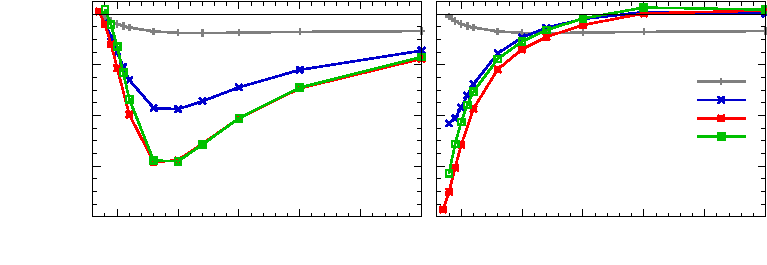
\includegraphics[width={368.00bp},height={127.00bp}]{Figs/scan_DBS}}%
    \gplfronttext
  \end{picture}%
\endgroup

		\end{column}
		\hspace{40pt}
		\begin{column}{0.3\textwidth}
			\centering
	 		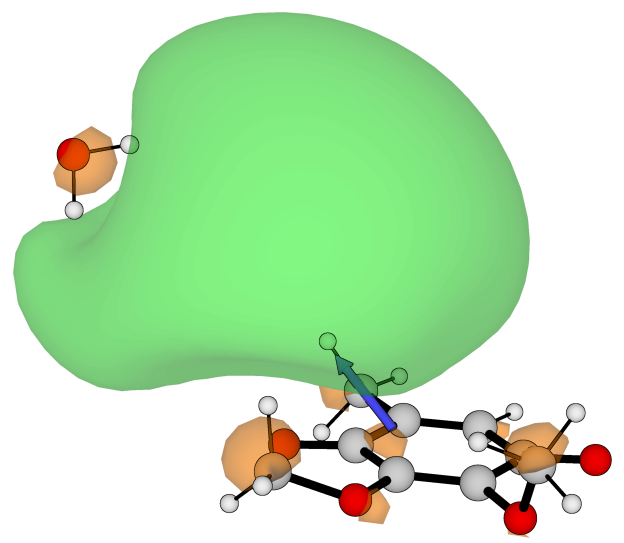
\includegraphics[width=0.6\textwidth]{Figs/Q0_H2O_H.png}\\
			\vfill
			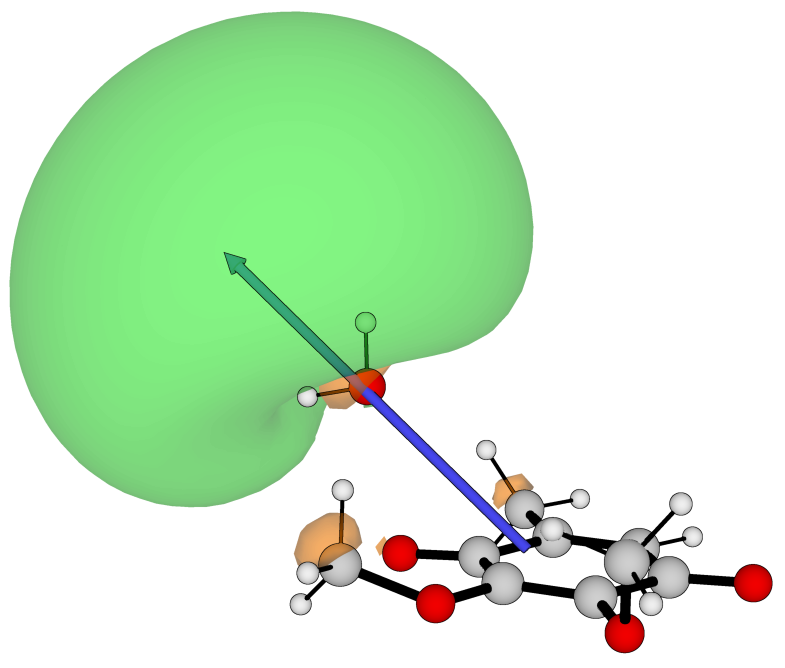
\includegraphics[width=0.6\textwidth]{Figs/Q0_H2O_O.png}	
		\end{column}
	\end{columns}		
\end{frame}

\begin{frame}
	\frametitle{\huge Interaction with solvent molecules (VBS)}\large
	%A directed interaction with small molecules strongly stabilises the VBS.\\
	\begin{itemize}
		\item \textbf{Antiparallel dipoles}: VBS strongly stabilised at short distances.
		\item \textbf{Aligned dipoles}: VBS destabilised.
		\item Intermolecular interactions larger effect on VBS than methoxy chain rotations.
	\end{itemize}
	\vspace{5pt}
	\begin{columns}[c]
		\begin{column}{0.7\textwidth}
			\centering
			\small	
			% GNUPLOT: LaTeX picture with Postscript
\begingroup
  \makeatletter
  \providecommand\color[2][]{%
    \GenericError{(gnuplot) \space\space\space\@spaces}{%
      Package color not loaded in conjunction with
      terminal option `colourtext'%
    }{See the gnuplot documentation for explanation.%
    }{Either use 'blacktext' in gnuplot or load the package
      color.sty in LaTeX.}%
    \renewcommand\color[2][]{}%
  }%
  \providecommand\includegraphics[2][]{%
    \GenericError{(gnuplot) \space\space\space\@spaces}{%
      Package graphicx or graphics not loaded%
    }{See the gnuplot documentation for explanation.%
    }{The gnuplot epslatex terminal needs graphicx.sty or graphics.sty.}%
    \renewcommand\includegraphics[2][]{}%
  }%
  \providecommand\rotatebox[2]{#2}%
  \@ifundefined{ifGPcolor}{%
    \newif\ifGPcolor
    \GPcolortrue
  }{}%
  \@ifundefined{ifGPblacktext}{%
    \newif\ifGPblacktext
    \GPblacktexttrue
  }{}%
  % define a \g@addto@macro without @ in the name:
  \let\gplgaddtomacro\g@addto@macro
  % define empty templates for all commands taking text:
  \gdef\gplbacktext{}%
  \gdef\gplfronttext{}%
  \makeatother
  \ifGPblacktext
    % no textcolor at all
    \def\colorrgb#1{}%
    \def\colorgray#1{}%
  \else
    % gray or color?
    \ifGPcolor
      \def\colorrgb#1{\color[rgb]{#1}}%
      \def\colorgray#1{\color[gray]{#1}}%
      \expandafter\def\csname LTw\endcsname{\color{white}}%
      \expandafter\def\csname LTb\endcsname{\color{black}}%
      \expandafter\def\csname LTa\endcsname{\color{black}}%
      \expandafter\def\csname LT0\endcsname{\color[rgb]{1,0,0}}%
      \expandafter\def\csname LT1\endcsname{\color[rgb]{0,1,0}}%
      \expandafter\def\csname LT2\endcsname{\color[rgb]{0,0,1}}%
      \expandafter\def\csname LT3\endcsname{\color[rgb]{1,0,1}}%
      \expandafter\def\csname LT4\endcsname{\color[rgb]{0,1,1}}%
      \expandafter\def\csname LT5\endcsname{\color[rgb]{1,1,0}}%
      \expandafter\def\csname LT6\endcsname{\color[rgb]{0,0,0}}%
      \expandafter\def\csname LT7\endcsname{\color[rgb]{1,0.3,0}}%
      \expandafter\def\csname LT8\endcsname{\color[rgb]{0.5,0.5,0.5}}%
    \else
      % gray
      \def\colorrgb#1{\color{black}}%
      \def\colorgray#1{\color[gray]{#1}}%
      \expandafter\def\csname LTw\endcsname{\color{white}}%
      \expandafter\def\csname LTb\endcsname{\color{black}}%
      \expandafter\def\csname LTa\endcsname{\color{black}}%
      \expandafter\def\csname LT0\endcsname{\color{black}}%
      \expandafter\def\csname LT1\endcsname{\color{black}}%
      \expandafter\def\csname LT2\endcsname{\color{black}}%
      \expandafter\def\csname LT3\endcsname{\color{black}}%
      \expandafter\def\csname LT4\endcsname{\color{black}}%
      \expandafter\def\csname LT5\endcsname{\color{black}}%
      \expandafter\def\csname LT6\endcsname{\color{black}}%
      \expandafter\def\csname LT7\endcsname{\color{black}}%
      \expandafter\def\csname LT8\endcsname{\color{black}}%
    \fi
  \fi
    \setlength{\unitlength}{0.0500bp}%
    \ifx\gptboxheight\undefined%
      \newlength{\gptboxheight}%
      \newlength{\gptboxwidth}%
      \newsavebox{\gptboxtext}%
    \fi%
    \setlength{\fboxrule}{0.5pt}%
    \setlength{\fboxsep}{1pt}%
    \definecolor{tbcol}{rgb}{1,1,1}%
\begin{picture}(7360.00,2540.00)%
    \gplgaddtomacro\gplbacktext{%
      \csname LTb\endcsname%%
      \put(782,453){\makebox(0,0)[r]{\strut{}-2.0}}%
      \csname LTb\endcsname%%
      \put(782,798){\makebox(0,0)[r]{\strut{}-1.9}}%
      \csname LTb\endcsname%%
      \put(782,1142){\makebox(0,0)[r]{\strut{}-1.8}}%
      \csname LTb\endcsname%%
      \put(782,1486){\makebox(0,0)[r]{\strut{}-1.7}}%
      \csname LTb\endcsname%%
      \put(782,1831){\makebox(0,0)[r]{\strut{}-1.6}}%
      \csname LTb\endcsname%%
      \put(782,2175){\makebox(0,0)[r]{\strut{}-1.5}}%
      \csname LTb\endcsname%%
      \put(782,2519){\makebox(0,0)[r]{\strut{}-1.4}}%
      \csname LTb\endcsname%%
      \put(1114,277){\makebox(0,0){\strut{}$5$}}%
      \csname LTb\endcsname%%
      \put(1699,277){\makebox(0,0){\strut{}$10$}}%
      \csname LTb\endcsname%%
      \put(2283,277){\makebox(0,0){\strut{}$15$}}%
      \csname LTb\endcsname%%
      \put(2868,277){\makebox(0,0){\strut{}$20$}}%
      \csname LTb\endcsname%%
      \put(3452,277){\makebox(0,0){\strut{}$25$}}%
      \csname LTb\endcsname%%
      \put(4036,277){\makebox(0,0){\strut{}$30$}}%
      \csname LTb\endcsname%%
      \put(2458,660){\makebox(0,0){\strut{}VBS Antiparallel}}%
    }%
    \gplgaddtomacro\gplfronttext{%
      \csname LTb\endcsname%%
      \put(229,1486){\rotatebox{-270.00}{\makebox(0,0){\strut{}Energy (eV)}}}%
      \csname LTb\endcsname%%
      \put(2458,13){\makebox(0,0){\strut{}Distance (\AA)}}%
    }%
    \gplgaddtomacro\gplbacktext{%
      \csname LTb\endcsname%%
      \put(4085,453){\makebox(0,0)[r]{\strut{}}}%
      \csname LTb\endcsname%%
      \put(4085,798){\makebox(0,0)[r]{\strut{}}}%
      \csname LTb\endcsname%%
      \put(4085,1142){\makebox(0,0)[r]{\strut{}}}%
      \csname LTb\endcsname%%
      \put(4085,1486){\makebox(0,0)[r]{\strut{}}}%
      \csname LTb\endcsname%%
      \put(4085,1831){\makebox(0,0)[r]{\strut{}}}%
      \csname LTb\endcsname%%
      \put(4085,2175){\makebox(0,0)[r]{\strut{}}}%
      \csname LTb\endcsname%%
      \put(4085,2519){\makebox(0,0)[r]{\strut{}}}%
      \csname LTb\endcsname%%
      \put(4417,277){\makebox(0,0){\strut{}$5$}}%
      \csname LTb\endcsname%%
      \put(5002,277){\makebox(0,0){\strut{}$10$}}%
      \csname LTb\endcsname%%
      \put(5586,277){\makebox(0,0){\strut{}$15$}}%
      \csname LTb\endcsname%%
      \put(6171,277){\makebox(0,0){\strut{}$20$}}%
      \csname LTb\endcsname%%
      \put(6755,277){\makebox(0,0){\strut{}$25$}}%
      \csname LTb\endcsname%%
      \put(7339,277){\makebox(0,0){\strut{}$30$}}%
      \csname LTb\endcsname%%
      \put(5761,660){\makebox(0,0){\strut{}VBS Parallel}}%
    }%
    \gplgaddtomacro\gplfronttext{%
      \csname LTb\endcsname%%
      \put(6584,2361){\makebox(0,0)[r]{\strut{}$\mathrm{CH}_4$}}%
      \csname LTb\endcsname%%
      \put(6584,2185){\makebox(0,0)[r]{\strut{}$\mathrm{NH}_3$}}%
      \csname LTb\endcsname%%
      \put(6584,2009){\makebox(0,0)[r]{\strut{}$\mathrm{H}_2\mathrm{O}$}}%
      \csname LTb\endcsname%%
      \put(6584,1833){\makebox(0,0)[r]{\strut{}$\mathrm{HF}$}}%
      \csname LTb\endcsname%%
      \put(5761,13){\makebox(0,0){\strut{}Distance (\AA)}}%
    }%
    \gplbacktext
    \put(0,0){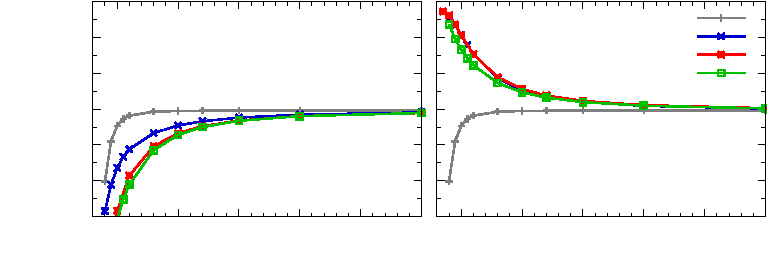
\includegraphics[width={368.00bp},height={127.00bp}]{Figs/scan_VBS}}%
    \gplfronttext
  \end{picture}%
\endgroup

		\end{column}
		\hspace{40pt}
		\begin{column}{0.3\textwidth}
			\centering
	 		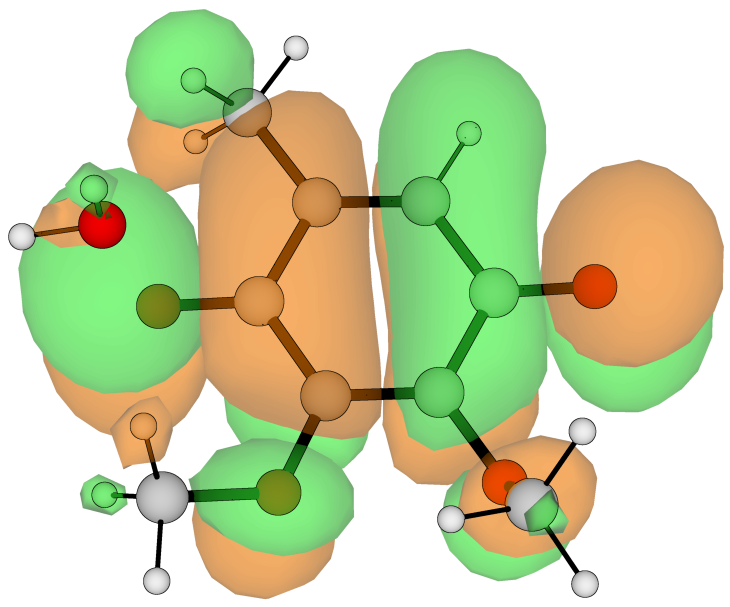
\includegraphics[width=0.6\textwidth]{Figs/Q0_H2O_VBS.png}\\
			\vfill
			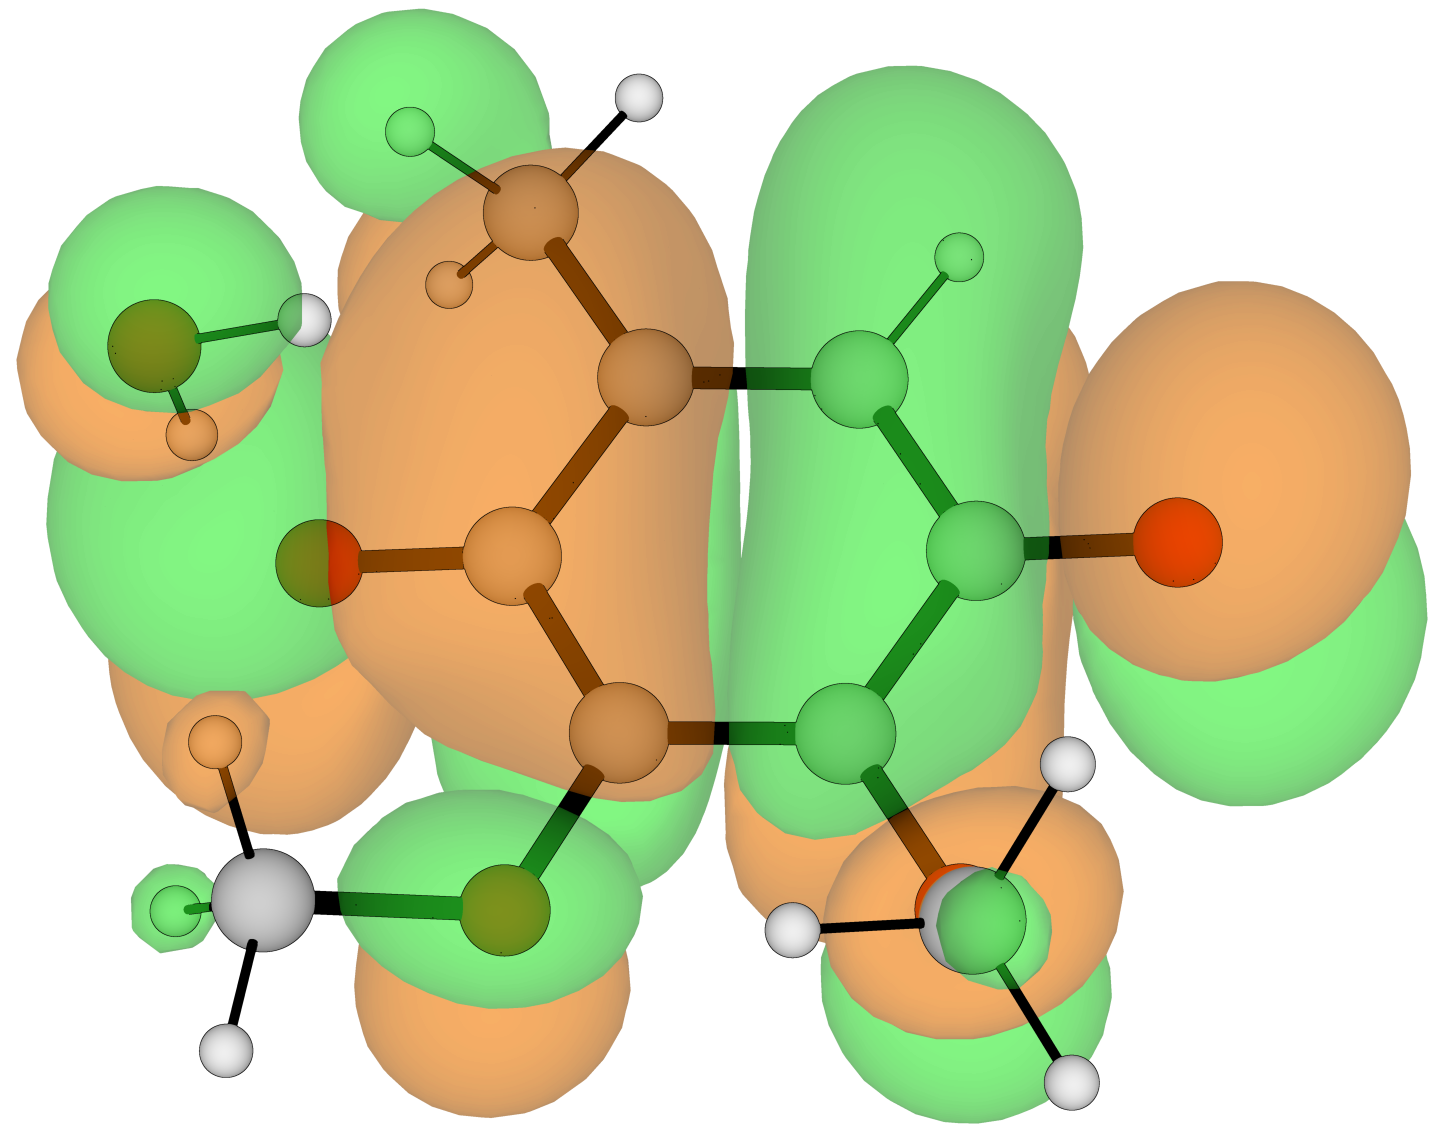
\includegraphics[width=0.6\textwidth]{Figs/Q0_H2O_H_VBS.png}	
		\end{column}
	\end{columns}		
\end{frame}

\section{Conclusions}
\begin{frame}{\huge Conclusions}\large
	\begin{itemize}
		%\item EA-EOM-CC2 is suitable for DBS; diffuse functions are critical. VBS energies are consistently overbound.
		%\item EOM-CC2 Dyson orbitals implemented in Q-Chem show good agreement with EOM-CCSD.
		\item Methoxy chain rotation in Q0 and Q1 significantly alters dipole moment, VBS, and DBS energies.
		\item In general, DBS electron binding energy isloosely correlated with dipole strength.
		\item For equivalent conformers, the correlation can be very strong
		\item Solvent interactions dramatically affect VBS and DBS stability
		\item Intermolecular interactions larger effect on VBS than methoxy chain rotations.
	\end{itemize}	
	\centering
	\vspace{40pt}
	\Huge \textcolor{kul-blue}{\textbf{Thanks for your attention!}}
\end{frame}

\appendix

\begin{frame}{\huge Acknowledgements}\large
	\centering
	\begin{columns}
		\begin{column}[c]{0.48\textwidth}
			\centering
			\vfill
			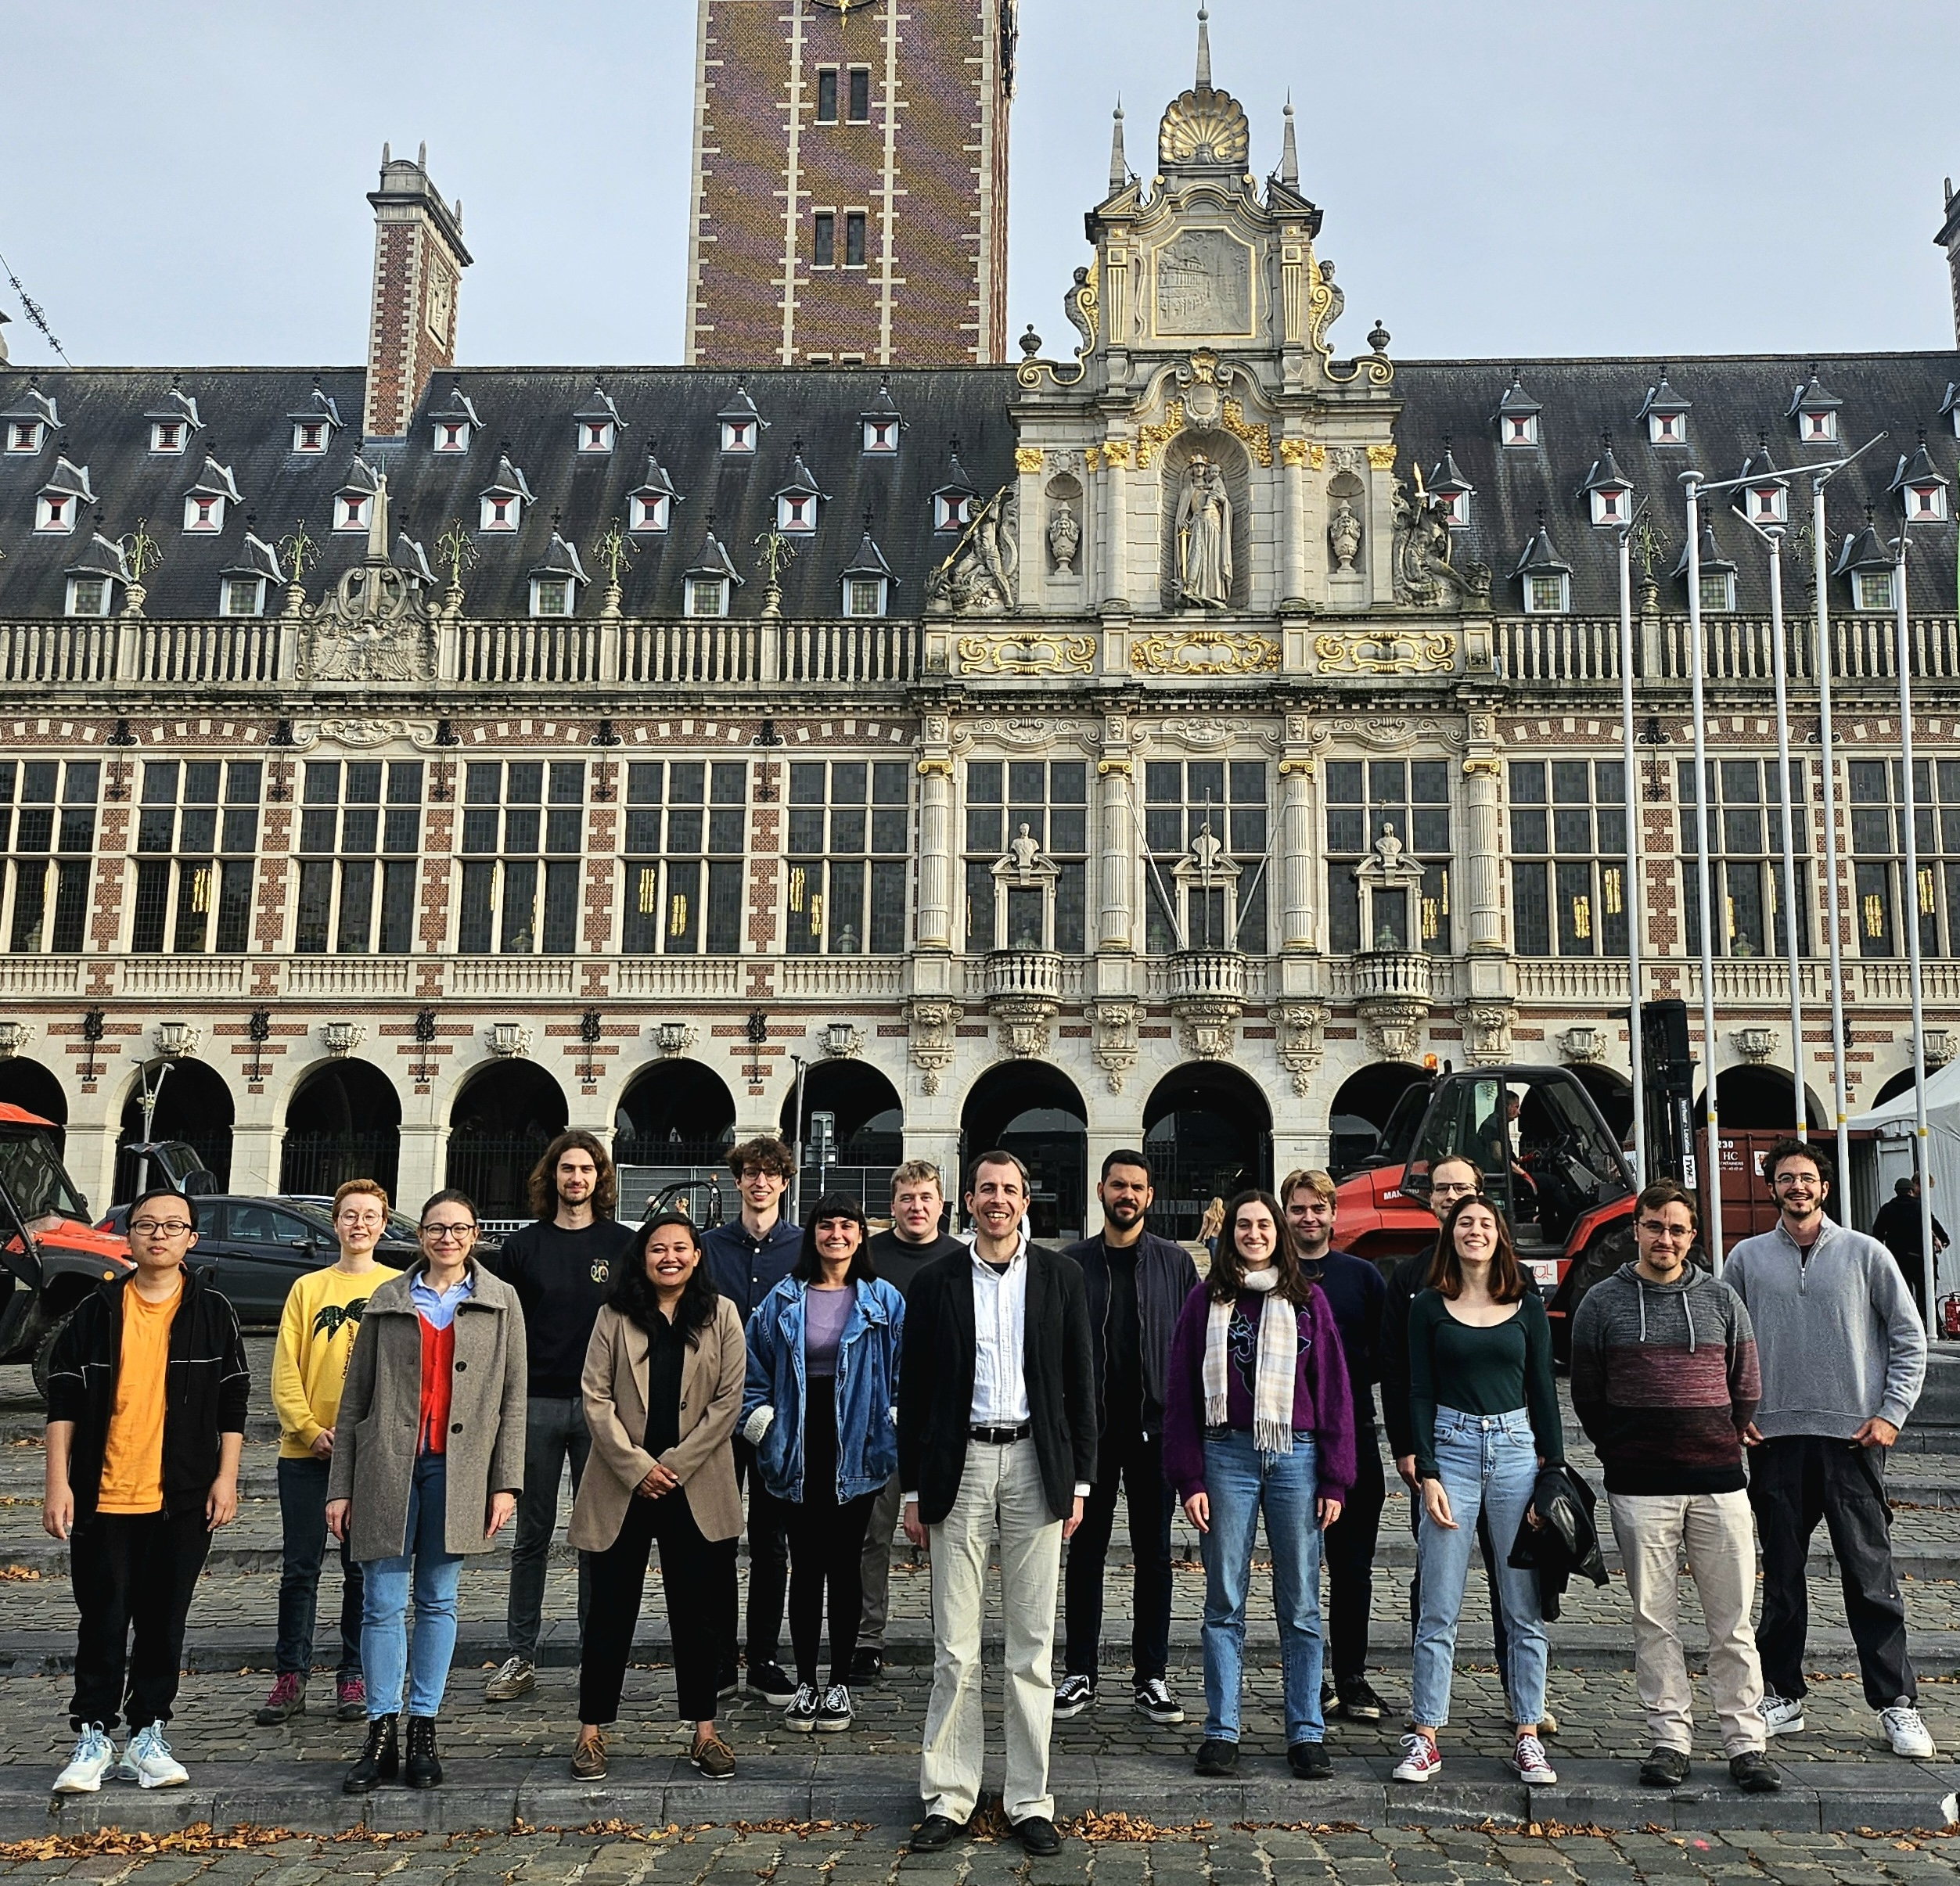
\includegraphics[width=\textwidth]{Figs/TJ.jpeg}
			\vfill
		\end{column}
		\begin{column}[c]{0.3\textwidth}
			\centering
			
\includegraphics[width=0.45\textwidth]{Figs/La-Caixa.png}\\\vfill
			
\includegraphics[width=0.5\textwidth]{Figs/erc.png}\\\vfill
			
\includegraphics[width=\textwidth]{Figs/VSC-Combilogo.png}\\\vfill
			%
\includegraphics[width=0.8\textwidth]{Figs/QCLogo.png}\\\vfill
		\end{column}
	\end{columns}

	\vspace{3pt}
\end{frame}

\begin{frame}{\huge DBS Basis set convergence}\normalsize
	\vspace{-20pt}
	\begin{table}[p]
	\centering
	\caption{ Electron affinity of dipole-bound radical anions computed using different augmented Dunning basis sets and EOM-EA RI-CC2 and EOM-EA RI-CCSD. Koopman' theorem (KT), and dipole moment, \textmu, calculated at the HF/aug-cc-pVTZ+6s3p level, and mean absolute error (MAE) taking CCSD/aug-cc-pVTZ+6s3p as reference are also given. The values are in meV and Debye respectively.}
	\footnotesize
	\vspace{-5pt}
	\begin{tabular}{cccccccccccc}
		\toprule
		& & \multicolumn{6}{c}{RI-CC2} & \multicolumn{2}{c}{RI-CCSD} & & \\
		\cmidrule(lr){3-8} \cmidrule(lr){9-10} 
		& & \multicolumn{4}{c}{aug-cc-pVTZ} & pVDZ & pVQZ & pVDZ & pVTZ & & \\
		\multicolumn{2}{c}{Molecule} & 2s1p & 4s2p & 6s3p & 8s4p & 6s3p & 6s3p & 6s3p & 6s3p & KT & \textmu \\
		\hline
		Acetaldehyde & \ce{CH3CHO} & -156.7 & -27.8 & -3.2 & 0.8 & -4.6 & -3.2 & -4.6 & -3.1 & -0.4 & 3.29 \\
		Acetone & \ce{(CH3)2CO} & -114.9 & -16.8 & 1.3 & 3.3 & -0.3 & 0.9 & -0.5 & 0.9 & -5.1 & 3.46 \\
		Acetonitrile & \ce{CH3CN} & -61.2 & 12.6 & 19.9 & 20.1 & 18.2 & 20.3 & 17.1 & 18.4 & 4.2 & 4.29 \\
		Benzaldehyde & \ce{C6H5CHO} & -97.1 & -2.1 & 8.9 & 9.6 & 7.4 & 9.1 & 3.4 & 4.6 & -4.9 & 3.77 \\
		N,N-Dimethylformamide & \ce{(CH3)2NCHO} & -81.1 & 5.4 & 14.1 & 14.4 & 13.2 & 14.4 & 13.3 & 13.7 & 1.9 & 4.48 \\
		DMSO & \ce{(CH3)2SO} & -84.5 & 4.0 & 15.4 & 16.1 & 14.8 & 15.5 & 14.7 & 14.9 & 2.1 & 4.63 \\
		Formamide & \ce{CH3NO} & -92.2 & 1.1 & 16.2 & 17.2 & 15.1 & 17.0 & 15.1 & 15.9 & 3.4 & 4.28 \\
		Methylisocyanide & \ce{CH3NC} & -95.1 & -0.5 & 10.0 & 10.5 & 9.5 & 10.1 & 8.8 & 9.0 & -1.8 & 3.59 \\
		Nitrobenzene & \ce{C6H5NO2} & -63.6 & 30.6 & 34.8 & 34.8 & 32.5 & -- & 25.0 & 25.9 & 5.4 & 5.15 \\
		Nitromethane & \ce{CH3NO2} & -82.9 & 5.7 & 14.2 & 14.7 & 13.0 & 14.7 & 12.9 & 13.7 & 3.5 & 4.10 \\
		Nitrosobenzene & \ce{C6H5NO} & -125.0 & 1.0 & 11.4 & -- & 9.9 & -- & 5.1 & 6.0 & -4.1 & 3.73 \\
		Phenylisocyanide & \ce{C6H5NC} & -82.7 & 8.6 & 16.3 & 16.5 & 15.2 & 16.7 & 9.0 & 9.2 & -4.9 & 3.61 \\
		Pyridazine & \ce{C4H4N2} & -80.7 & 20.5 & 26.3 & 26.4 & 25.0 & 26.7 & 18.6 & 19.1 & 1.7 & 4.41 \\
		Vinylene carbonate & \ce{C3H2O3} & -82.5 & 20.9 & 27.2 & 27.4 & 26.4 & 27.7 & 25.1 & 25.5 & 10 & 5.05 \\
		\cmidrule(lr){2-11} 
		& MAE & 105.3 & 8.8 & 2.8 & 3.4 & 2.3 & 2.4 & 0.8 & 0.0 & 12.0 & \\
		\bottomrule
	\end{tabular}
	\end{table}
\end{frame}

\iffalse

% --- New Slide: How do we treat electronic structure theoretically? ---

\begin{frame}{\huge Theoretical treatment of electronic structure}\large
    \vspace{5pt}
    \begin{itemize}
        \item Quantum chemistry describes molecules by solving the Schrödinger equation for electrons and nuclei.
        \item Approximations are needed for all but the smallest systems.
        \item \textbf{Key concepts:}
        \begin{itemize}
            \item Molecular orbitals
            \item Electron correlation
            \item Basis sets
        \end{itemize}
    \end{itemize}
    \vspace{5pt}
    \centering
    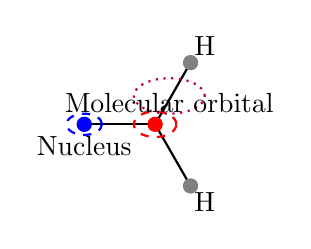
\begin{tikzpicture}[scale=0.9]
        % Draw molecule
        \draw[thick] (0,0) -- (1,0);
        \draw[thick] (1,0) -- (1.5,0.87);
        \draw[thick] (1,0) -- (1.5,-0.87);
        \filldraw[blue] (0,0) circle (0.1);
        \filldraw[red] (1,0) circle (0.1);
        \filldraw[gray] (1.5,0.87) circle (0.1);
        \filldraw[gray] (1.5,-0.87) circle (0.1);
        % Draw orbitals
        \draw[thick, dashed, blue] (0,0) ellipse (0.25 and 0.15);
        \draw[thick, dashed, red] (1,0) ellipse (0.3 and 0.18);
        % Electron cloud
        \draw[thick, dotted, purple] (1.2,0.4) ellipse (0.5 and 0.25);
        % Labels
        \node at (0,-0.3) {Nucleus};
        \node at (1.7,1.1) {H};
        \node at (1.7,-1.1) {H};
        \node at (1.2,0.3) {Molecular orbital};
    \end{tikzpicture}
\end{frame}

\begin{frame}{\huge CC2}\large
	Second-order approximate coupled-cluster singles and doubles (CC2) method is obtained from a perturbative analysis of the CCSD model
	\vspace{5pt}
	\begin{itemize}
		\item Lowers computational scaling from CCSD 
		\item Allows treatment of “big” molecules: $>$ 25 heavy atoms
	\end{itemize}
	\centering
	\vspace{30pt}
	\begin{table}
		\centering
		\begin{tabular}{lcc}\toprule
		\textbf{Method} & \textbf{Scaling} & \textbf{Memory}\\\midrule
		CCSD & $O(N^6)$ & $O(N^{4})^*$\\
		CC2 & $O(N^5)$ & $O(N^{4})^*$\\\bottomrule
		\multicolumn{3}{l}{\small $^*\,O(N^3)$ with RI approximation.}
		\end{tabular}
	\end{table}
\end{frame}

\begin{frame}{\huge Quantum chemical methods}\large
	The time independent Schrödinger equation is approximatelly solved to describe the electronic structure of molecules:
	\begin{equation*}
		\hat{H} \Psi = E \Psi
	\end{equation*}
	We construct the wavefunction $\Psi$ as a combination of molecular orbitals (MOs):
	\begin{equation*}
		\Psi = \sum_{i} c_i \phi_i
	\end{equation*}
\end{frame}
\fi

\end{document}
